\section{张量运算}\label{chapter:operations}
回顾一下，张量 $\Tt \in \RR^{d_1 \times \cdots \times d_N}$ 可以看作一个 $N$ 阶多维数组：$N$ 阶（亦称 $N$ 路）张量有 $N$ 个模，每个模对应一个维度 \citep{kolda2009tensor}。
\paragraph{张量纤维} 对任意模 $i$（其中 $i = 1, \dots, N$），将除第 $i$ 个以外的指标全部固定，便得到张量的\textit{纤维}。例如，矩阵的一列对应模 1 纤维，而矩阵的一行对应模 2 纤维。在三阶张量 $\Tt \in \RR^{d_1 \times d_2 \times d_3}$ 中，模 1 纤维有 $d_2d_3$ 个，它们是尺寸为 $d_1$ 的向量，即对 $i_2 \in [d_2]$ 与 $i_3 \in [d_3]$，有 $\Tt_{:,i_2,i_3} \in \RR^{d_1}$。冒号表示第一个指标变化，而 $i_2$ 与 $i_3$ 保持固定。纤维是向量。
\paragraph{张量切片} 张量的切片是将除两个指标以外的所有指标固定后得到的二维数组（矩阵）。对三阶张量 $\Tt \in \RR^{d_1 \times d_2 \times d_3}$，分别有水平切片、侧面切片与正面切片，记为 $\Tt_{i_1,:,:} \in \RR^{d_2 \times d_3}$、$\Tt_{:,i_2,:} \in \RR^{d_1 \times d_3}$ 与 $\Tt_{:,:,i_3} \in \RR^{d_1 \times d_2}$。因此，切片是矩阵。
\paragraph{标量乘法} 
设 $\lambda \in \RR$ 为标量。标量乘积 $\lambda\Tt$ 
 仍是维度为 $d_1 \times \cdots \times d_N$ 的张量，逐元素定义为：
$
    (\lambda\Tt)_{i_1 \cdots i_N} = \lambda \cdot \Tt_{i_1 \cdots i_N}$
对所有可取的指标 $i_k\in[d_k]$ 与 $k\in[N]$。
\paragraph{张量求和} 设 $\St\in\RR^{d_1\times\cdots\times d_N}$。张量 $\Tt$ 与 $\St$ 之和仍是同维度的张量 $\Tt+\St\in\RR^{d_1\times\cdots\times d_N}$，逐元素定义为：$(\Tt+\St)_{i_1,\cdots,i_N} = \Tt_{i_1,\cdots,i_N} + \St_{i_1,\cdots,i_N}$，对所有可取的指标 $i_k\in[d_k]$ 与 $k\in[N]$。
\subsection{张量的置换与重排}
置换与重排是张量的两种基本运算。
\begin{itemize}
    \item \textbf{置换} 在不改变模的个数的情况下重新排列张量的指标。置换的一个常见例子是矩阵转置。
    \item  \textbf{重排} 把多个指标合并为较大的指标，或把一个较大的指标拆分为多个较小的指标，从而减少或增加指标的总数，同时保持张量的总体尺寸不变。
\end{itemize}
下面介绍矩阵化（matricization）与向量化（vectorization）这两种常见的张量重排运算。
\begin{definition}（矩阵化）\label{matricizitation:def}
设 $\Tt\in\RR^{d_1\times d_2\times \cdots\times d_N}$。对 $n\in[N]$，把 $\Tt$ 的所有模 $n$ 纤维取出并按列堆叠，即可展开为矩阵 $\Tt_{(n)}\in\RR^{d_n\times d_1d_2\cdots d_{n-1}d_{n+1}\cdots d_N}$，称为模 $n$ 矩阵化。例如，张量 $\Tt\in\RR^{d_1\times d_2\times d_3}$ 沿模 $1$ 的矩阵化记作 $\Tt_{(1)}$，它是如下所示的 $d_1\times d_2d_3$ 矩阵
$$
    \begin{bmatrix}
    \vline & \vline & \vline  & \vline \\
    \Tt_{:,1,1} & {\Tt}_{:,1,2}  & \dots  & {\Tt}_{:,d_2,d_3} \\
    \vline & \vline & \vline  & \vline 
    \end{bmatrix}
\in\RR^{d_1\times d_2d_3}.
$$

模 2 与模 3 矩阵化 $\Tt_{(2)}\in\RR^{d_2\times d_1d_3}$ 和 $\Tt_{(3)}\in\RR^{d_3\times d_1d_2}$ 的定义类似。
\end{definition}

注意，在模 1 矩阵化中，对应于 $\Tt$ 的第二和第三个模的两个指标被归并在一起，形成一个取值从 1 到 $d_2d_3$ 的新指标。在前面的定义中，我们选择按字典序排列这个新指标，例如当 $d_2=d_3=3$ 时为 $11,12,13,21,22,23,31,32,33$。矩阵化中各列的排列次序有时也采用别的约定~（例如 \citep{kolda2009tensor} 中的逆字典序）。一般说来，具体采用哪一种排列
并不重要，但在相关的计算中必须保持一致~（详见 \citep{kolda2006multilinear}）。



在张量网络图中，我们通过把相应的边合并到一起来表示这种指标归并：
$$\Tt_{(1)} = 
\left(\begin{tikzpicture}[baseline=\baseline]
    \tikzset{tensor/.style = {minimum size = 0.5cm,shape = circle,thick,draw=black,inner sep = 0pt}, edge/.style = {thick,line width=.4mm},every loop/.style={}}
    \def\y{0}
    \def\x{0}
    \node[tensor,fill=red!50!white] (T) at (\x,\y){\scalebox{0.85}{$\Tt$}};
    \draw[edge] (T) -- (\x+0.7,\y) node [midway,above]{\scalebox{0.7}{\dimcolor{$d_2$}}};
    \draw[edge] (T) -- (\x-0.7,\y) node [midway,above]{\scalebox{0.7}{\dimcolor{$d_1$}}};
    \draw[edge] (T) -- (\x,\y-0.7) node [midway,left]{\scalebox{0.7}{\dimcolor{$d_3$}}}; 
\end{tikzpicture}\right)_{(1)}
=
\begin{tikzpicture}[baseline=\baseline]
    \tikzset{tensor/.style = {minimum size = 0.5cm,shape = circle,thick,draw=black,inner sep = 0pt}, edge/.style = {thick,line width=.4mm},every loop/.style={}}
    \def\y{0}
    \def\x{0}
    \node[tensor,fill=red!50!white] (A) at (\x,\y){\scalebox{0.85}{$\Tt$}};
    \draw[edge] (\x+0.2,\y+0.15) -- (\x+0.5,\y+0.15)-- (\x+0.5,\y+0.05) -- (\x+1,\y+0.05) node [midway,above]
    {\scalebox{0.7}{\dimcolor{$d_2$}}};
    \draw[edge] (\x+0.2,\y-0.15) -- (\x+0.5,\y-0.15)-- (\x+0.5,\y-0.05)-- (\x+1,\y-0.05) node [midway,below]
    {\scalebox{0.7}{\dimcolor{$d_3$}}};
    \draw[edge] (A) -- (\x-0.7,\y)node [midway,above]
    {\scalebox{0.7}{\dimcolor{$d_1$}}};
\end{tikzpicture}
=
\begin{tikzpicture}[baseline=\baseline]
    \tikzset{tensor/.style = {minimum size = 0.5cm,shape = circle,thick,draw=black,inner sep = 0pt}, edge/.style = {thick,line width=.4mm},every loop/.style={}}
    \def\y{0}
    \def\x{0}
    \node[tensor,fill=red!50!white] (T) at (\x,\y){\scalebox{0.85}{$\Tt$}};
    \draw[edge](T) -- (\x+1,\y) node [midway, above]{\scalebox{0.7}{\dimcolor{$d_2d_3$}}};
    \draw[edge](T) -- (\x-1,\y) node [midway, above]{\scalebox{0.7}{\dimcolor{$d_1$}}};
\end{tikzpicture}
\in\RR^{d_1\times d_2d_3}.
$$
可以看到，形如
$\begin{tikzpicture}[baseline=\baseline]
    \tikzset{tensor/.style = {minimum size = 0.5cm,shape = circle,thick,draw=black,inner sep = 0pt}, edge/.style = {thick,line width=.4mm},every loop/.style={}}
    \def\y{0}
    \def\x{0}
    \draw[edge] (\x+0.15,\y+0.2) -- (\x+0.5,\y+0.2) -- (\x+0.5,\y+0.1) -- (\x+1,\y+0.1) node [midway,above]
    {\scalebox{0.7}{\dimcolor{$d_2$}}};
    \draw[edge] (\x+0.15,\y-0.1) -- (\x+0.5,\y-0.1)-- (\x+0.5,\y)-- (\x+1,\y) 
node [midway,below]
    {\scalebox{0.7}{\dimcolor{$d_3$}}};
    \end{tikzpicture}
$
的归并腿在张量网络图中表示一条大小为 $d_2d_3$ 的边。


一般地，矩阵化的概念可以推广到 $\Tt$ 的模的任一子集 $I\subset [N]$：把属于 $I$ 的模映为行，把不属于 $I$ 的模映为列，从而得到大小为 $\prod_{i\in I} d_i \times \prod_{j\in [N]\setminus I} d_j$ 的矩阵 $\Tt_{(I)}$。例如，对六阶张量 $\Tt\in\RR^{d_1\times\dots\times d_6}$，可以按如下方式归并指标：
\begin{align*}
\Tt_{i_1,\dots,i_6} 
&=
\begin{tikzpicture}[baseline=\baseline]
    \tikzset{tensor/.style = {minimum size = 0.5cm,shape = circle,thick,draw=black,inner sep = 0pt}, edge/.style = {thick,line width=.4mm},every loop/.style={}}
    \def\y{0}
    \def\x{0}
    \node[tensor,fill=red!20!blue!40!white] (T) at (\x,\y){\scalebox{0.85}{$\Tt$}};
    \draw[edge] (T) -- (\x+0.85,\y) node [very near end,right]
    {\scalebox{0.7}{\indcolor{$i_4$}}};
    \draw[edge] (T) -- (\x,\y-0.85) node [very near end, below]
    {\scalebox{0.7}{\indcolor{$i_6$}}};
    \draw[edge] (T) -- (\x-0.85,\y)node [very near end,left]
    {\scalebox{0.7}{\indcolor{$i_1$}}};
    \draw[edge] (T) -- (\x,\y+0.85) node [very near end,above]
    {\scalebox{0.7}{\indcolor{$i_3$}}};
    \draw[edge] (T) -- (\x-0.75,\y+0.5) node [pos=1.3]
    {\scalebox{0.7}{\indcolor{$i_2$}}};
    \draw[edge] (T) -- (\x+0.75,\y-0.5) node [pos=1.3]
    {\scalebox{0.7}{\indcolor{$i_5$}}};
    \node[draw=none] at (\x+2,\y+0.2){$\underrightarrow{I=\{1,2,6\}}$};
    \end{tikzpicture}
\begin{tikzpicture}[baseline=\baseline]
    \tikzset{tensor/.style = {minimum size = 0.5cm,shape = circle,thick,draw=black,inner sep = 0pt}, edge/.style = {thick,line width=.4mm},every loop/.style={}}
    \def\y{0}
    \def\x{0}
    \node[tensor,fill=red!20!blue!40!white] (T) at (\x,\y){\scalebox{0.85}{$\Tt$}};
    \draw[edge](T) -- (\x+0.85,\y)node [very near end, right]{\scalebox{0.7}{\indcolor{$i_5$}}};
    \draw[edge](\x+0.16,\y+0.2) -- (\x+0.5,\y+0.2) -- (\x+0.5,\y+0.1) -- (\x+0.85,\y+0.1)node [very near end, above]{\scalebox{0.7}{\indcolor{$i_3$}}};
    \draw[edge](\x+0.16,\y-0.2) -- (\x+0.5,\y-0.2) -- (\x+0.5,\y-0.1) -- (\x+0.85,\y-0.1)node [very near end, below]{\scalebox{0.7}{\indcolor{$i_4$}}};
    \draw[edge](T) -- (\x-0.85,\y)node [very near end, left]{\scalebox{0.7}{\indcolor{$i_2$}}};
    \draw[edge](\x-0.16,\y+0.2) -- (\x-0.5,\y+0.2) -- (\x-0.5,\y+0.1) -- (\x-0.85,\y+0.1)node [very near end, above]{\scalebox{0.7}{\indcolor{$i_6$}}};
    \draw[edge](\x-0.16,\y-0.2) -- (\x-0.5,\y-0.2) -- (\x-0.5,\y-0.1) -- (\x-0.85,\y-0.1)node [very near end, below]{\scalebox{0.7}{\indcolor{$i_1$}}};
\end{tikzpicture}\\
&=
(\Tt_{(\{1,2,6\})})_{i_1i_2i_6 , i_3i_4i_5}\in\RR^{d_1d_2d_6\times d_3d_4d_5}.
\end{align*}
这一概念虽然直观，写成形式化的记法却很繁琐：张量中属于 $I$ 的指标 $i_{r_1},i_{r_2},\cdots, i_{r_{|I|}}$（按降序排列）被映为行指标 $
j = 1+\sum_{l=1}^{|I|}
\left[(i_{r_l}-1)\prod_{m=1}^{l-1}I_{r_m}\right]
$，而其余指标 $i_{c_1},i_{c_2},\cdots, i_{c_{N-|I|}}$（同样按降序排列）被映为列指标 $k  = 1+\sum_{n=1}^{N - |I|}
\left[(i_{c_n}-1)\prod_{s=1}^{n-1}I_{r_s}\right]$。借助张量网络，我们只需把这类 
重排运算表示为边的归并，就能避开这种繁琐。 






与前面类似，张量既能转化为矩阵，也能转化为向量。这一过程称为向量化：
\begin{definition}（向量化）\label{def:vectorization}
设 $\Tt\in\RR^{d_1\times d_2\times\cdots\times d_N}$。$\Tt$ 的\emph{向量化}记为 $\vectorize(\Tt)\in\RR^{d_1d_2\cdots d_N}$，它是把自身的模 $N$ 纤维拼接起来所得到的向量\footnote{按字典序拼接。}。例如，张量 $\Tt\in\RR^{d_1\times d_2\times d_3}$ 的向量化为：
$$\vectorize(\Tt) =    
[(\Tt_{1,1,:})\ \  (\Tt_{1,2,:})\ \  \cdots \ \ (\Tt_{d_1,d_2,:})]^\ts
=
\begin{tikzpicture}[baseline=\baseline]
    \tikzset{tensor/.style = {minimum size = 0.5cm,shape = circle,thick,draw=black,inner sep = 0pt}, edge/.style = {thick,line width=.4mm},every loop/.style={}}
    \def\y{0}
    \def\x{0}
    \node[tensor,fill=blue!10!white] (A) at (\x,\y){\scalebox{0.85}{$\Tt$}};
    \draw[edge] (\x+0.15,\y+0.2) -- (\x+0.5,\y+0.2) -- (\x+0.5,\y+0.1) -- (\x+1,\y+0.1) node [midway,above]
    {\scalebox{0.7}{\dimcolor{$d_1$}}};
     \draw[edge] (A) -- (\x+1,\y)node [right]
    {\scalebox{0.7}{\dimcolor{$d_2$}}};

    \draw[edge] (\x+0.15,\y-0.2) -- (\x+0.5,\y-0.2)-- (\x+0.5,\y-0.1)-- (\x+1,\y-0.1) node [midway,below]
    {\scalebox{0.7}{\dimcolor{$d_3$}}};
    \end{tikzpicture}\in\RR^{d_1d_2d_3}.
$$
\end{definition}

向量化是一种展开操作，它把任意阶的张量化为向量。与矩阵化类似，在张量网络中，形如
$
\begin{tikzpicture}[baseline=\baseline]
    \tikzset{tensor/.style = {minimum size = 0.5cm,shape = circle,thick,draw=black,inner sep = 0pt}, edge/.style = {thick,line width=.4mm},every loop/.style={}}
    \def\y{0}
    \def\x{0}
    \draw[edge] (\x+0.15,\y+0.2) -- (\x+0.5,\y+0.2) -- (\x+0.5,\y+0.1) -- (\x+1,\y+0.1) node [midway,above]
    {\scalebox{0.7}{\textcolor{gray}{$d_1$}}};
    \draw[edge] (\x+0.15,\y) -- (\x+1,\y)node [right]
    {\scalebox{0.7}{\textcolor{gray}{$d_2$}}};
    \draw[edge] (\x+0.15,\y-0.2) -- (\x+0.5,\y-0.2)-- (\x+0.5,\y-0.1)-- (\x+1,\y-0.1) 
node [midway,below]
    {\scalebox{0.7}{\dimcolor{$d_3$}}};
    \end{tikzpicture}
$ 的边表示一条大小为 $d_1d_2d_3$ 的边。一般而言，全文中汇聚于一点的边表示一条边，其大小等于所有相关边大小之积。注意，张量的向量化等于该张量模 $1$ 矩阵化的向量化\footnote{为与本书所用的向量化定义保持一致，矩阵的向量化由其各行拼接而成，这有时称为\emph{行主序向量化}。注意，这正是 \textsf{Python} 中 \textsf{numpy} 包默认的向量化操作 \textsf{ravel()}。}，即对 $\Tt\in\RR^{d_1\times d_2\cdots \times d_N}$，有 $\vectorize(\Tt) = \vectorize(\Tt_{(1)})$。




\subsection{乘积}\label{sec:product}
张量可以用不同类型的运算组合起来，即进行各种\textit{乘法}。本节给出各类乘积运算的图示。
\paragraph{模 $n$ 张量乘积}\label{par:mode-n-tensor-product}
模 $n$ 乘积是张量沿某个特定的模与矩阵相乘，可视为矩阵乘法的推广。更确切地说，模 $n$ 乘积把矩阵与矩阵的乘法推广到某一个特定的模上，其中包括张量与矩阵、以及张量与向量之间的模 $n$ 乘积。
\begin{enumerate}
\item \textbf{模-n 乘积~（矩阵）。}\label{subsec:mode-n}
    张量 $\Xt\in\RR^{d_1\times\cdots\times d_N}$ 与矩阵 $\Mb\in\RR^{m\times d_n}$ 的模 $n$ 乘积记为
    $\Xt\ttm n \Mb \in \RR^{d_1\times \cdots\times d_{n-1}\times m\times d_{n+1}\times\cdots\times d_N}$，其定义为张量与矩阵沿张量的模 $n$、沿矩阵的第二模~（列指标）收缩，即 
    $$
  \Xt\ttm n \Mb
=
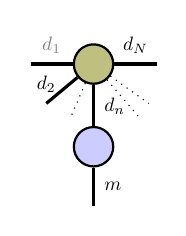
\begin{tikzpicture}[baseline=-0.5ex]
    \tikzset{tensor/.style = {minimum size = 0.5cm,shape = circle,thick,draw=black,inner sep = 0pt}, edge/.style = {thick,line width=.4mm},every loop/.style={}}
    \def\x{6}
    \node[tensor,fill=blue!20!white] (M) at (\x,-1.05) {$\Mb$};
    \node[tensor,fill=green!50!red!50!white] (At) at (\x,0) {$\Xt$};
    \draw[edge] (At) -- (\x-0.8,0) node [midway,above] {\scalebox{0.7}{\textcolor{gray}{$d_1$}}};
    \draw[edge] (At)-- (\x-0.6,-0.5) node [above]{\scalebox{0.7}{\dimcolor{$d_2$}}};
    \draw[edge] (At) -- (\x+0.8,0) node [midway,above] {\scalebox{0.7}{\dimcolor{$d_N$}}};;
    \draw[dotted] (At) -- (\x-0.3,-0.7);
    \draw[edge] (At) -- (\x,-0.8) node [midway,right] {\scalebox{0.7}{\dimcolor{$d_n$}}};
    \draw[dotted] (At) -- (\x+0.6,-0.7);
    \draw[dotted] (At) -- (\x+0.7,-0.5);
    \draw[edge] (M) -- (\x,-1.8) node [midway,right] {\scalebox{0.7}{\dimcolor{$m$}}};;
    \end{tikzpicture}
\in\RR^{d_1\times  \dots\times d_{n-1}\times m \times d_{n+1}\times \dots\times d_N}.
$$
该运算把张量的第 $n$ 模与矩阵的第二模~（列）收缩，原来的维数 $d_n$ 被新维数 $m$ 取代。若 $\Ab\in\RR^{d_n\times n},\Bb\in\RR^{d_m\times m}$ 与 $\Xt\in\RR^{d_1\times\cdots\times d_N}$ 所对应的模 $n\neq m$ 互不相同，则相乘的顺序无关紧要，即
$$
\Xt\ttm n \Ab \ttm m \Bb = 
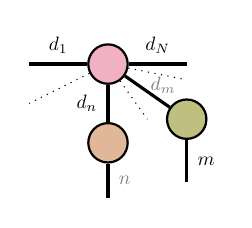
\begin{tikzpicture}[baseline=-0.5ex]
    \tikzset{tensor/.style = {minimum size = 0.5cm,shape = circle,thick,draw=black,inner sep = 0pt}, edge/.style = {thick,line width=.4mm},every loop/.style={}}
    \def\x{0}
    \def\y{0}
    \node[tensor,fill=blue!20!red!30!white] (Xt) at (\x,\y) {$\Xt$};
    \node[tensor,fill=green!30!red!40!white] (A) at (\x,\y-1) {$\Ab$};
    \node[tensor,fill=green!50!red!50!white] (B) at (\x+1,\y-0.7) {$\Bb$};
    \draw[edge] (Xt) -- (\x-1,\y) node [midway,above] {\scalebox{0.7}{\dimcolor{$d_1$}}};
    \draw[dotted] (Xt) -- (\x-1,\y-0.5);
    \draw[edge] (Xt) -- (\x+1,\y) node [midway,above] {\scalebox{0.7}{\dimcolor{$d_N$}}};
    \node[draw=none] () at (\x+0.7,\y-0.27) {\scalebox{0.7}{\textcolor{gray}{$d_m$}}};
    \draw[edge] (Xt) -- (A) node [midway,left] {\scalebox{0.7}{\dimcolor{$d_n$}}};
    \draw[edge] (A) -- (\x,\y-1.7) node [midway,right] {\scalebox{0.7}{\textcolor{gray}{$n$}}};
    \draw[edge] (Xt) -- (B);
    \draw[edge] (B) -- (\x+1,\y-1.5) node [midway,right] {\scalebox{0.7}{\dimcolor{$m$}}};
    \draw[dotted] (Xt) -- (\x+1,\y-0.2);
    \draw[dotted] (Xt) -- (\x+0.5,\y-0.7);
    \end{tikzpicture}
= \Xt\ttm m\Bb\ttm n \Ab,~~\text{For}~~n\neq m.
$$
然而当 $m = n$ 时，乘积的顺序就至关重要。特别地，若 $\Ab\in\RR^{n\times d_n}$、$\Bb\in\RR^{p\times n}$，则 $(\Xt\ttm n \Ab) \ttm n \Bb = \Xt\ttm n(\Bb\Ab)$，而乘积 $(\Xt\ttm n \Bb) \ttm n \Ab$ 仅当 $n=d_n=p$ 时才有意义。
模 $n$ 张量乘积可以视为经典矩阵乘法的推广。特别地，
用二阶张量的模 $1$ 乘积与模 $2$ 乘积即可还原出矩阵乘积：
若 $\Ab\in\RR^{m\times n}$、$\Bb\in\RR^{p\times n}$、$\Cb\in\RR^{d\times m}$，则
\begin{align*}
\Ab\ttm2 \Bb
=
\begin{tikzpicture}[baseline=\baseline]
   \tikzset{tensor/.style = {minimum size = 0.5cm,shape = circle,thick,draw=black,inner sep = 0pt}, edge/.style = {thick,line width=.4mm},every loop/.style={}}
    \def\y{0}
    \def\x{0}
    \node[tensor,fill=red!50!white] (A) at (\x,\y){\scalebox{0.85}{$\Ab$}};
    \node[tensor,fill=blue!50!white] (B) at (\x+1,\y){\scalebox{0.85}{$\Bb$}};
    \draw[edge] (A) -- (B) node [above,midway] {\scalebox{0.7}{\dimcolor{$n$}}};
    \draw[edge] (\x-0.25,\y) -- (\x-0.6,\y)  node [midway,above] {\scalebox{0.7}{\dimcolor{$m$}}};
    \draw[edge] (\x+1.25,\y) -- (\x+1.6,\y)  node [midway,above] {\scalebox{0.7}{\dimcolor{$p$}}};
    \end{tikzpicture}
    = \Ab\Bb^\ts\in\RR^{m\times p},
\end{align*}
\begin{align*}
    \Ab\ttm1 \Cb =
    \begin{tikzpicture}[baseline=\baseline]
   \tikzset{tensor/.style = {minimum size = 0.5cm,shape = circle,thick,draw=black,inner sep = 0pt}, edge/.style = {thick,line width=.4mm},every loop/.style={}}
    \def\y{0}
    \def\x{0}
    \node[tensor,fill=red!20!white] (C) at (\x,\y){\scalebox{0.85}{$\Cb$}};
    \node[tensor,fill=red!50!white] (A) at (\x+1,\y){\scalebox{0.85}{$\Ab$}};
    \draw[edge] (C) -- (A) node [above,midway] {\scalebox{0.7}{\dimcolor{$m$}}};
    \draw[edge] (\x-0.25,\y) -- (\x-0.6,\y)  node [midway,above] {\scalebox{0.7}{\dimcolor{$d$}}};
    \draw[edge] (\x+1.25,\y) -- (\x+1.6,\y)  node [midway,above] {\scalebox{0.7}{\dimcolor{$n$}}};
    \end{tikzpicture}
    = \Cb\Ab\in\RR^{d\times n}.
\end{align*}

下面的命题说明如何借助矩阵化与矩阵乘积来表示模 $n$ 乘积。
\begin{proposition}
设 $\Xt\in\RR^{d_1\times\dots\times d_N}$ 且 $\Mb\in\RR^{m\times d_n}$，则 
$(\Xt\ttm n \Mb)_{(n)} = \Mb\Xt_{(n)}$.
\begin{proof}
我们用一张简单的张量网络图来说明特殊情形 $n=2$、$N=3$ 下的这一恒等式，一般情形的推广是直接的。于是
\begin{align*}
(\Xt\ttm2\Mb)_{(2)} 
&= 
\left(
    \begin{tikzpicture}[baseline=\baseline]
    \tikzset{tensor/.style = {minimum size = 0.5cm,shape = circle,thick,draw=black,inner sep = 0pt}, edge/.style = {thick,line width=.4mm},every loop/.style={}}
    \def\y{0}
    \def\x{0}
    \node[tensor,fill=green!50!red!50!white] (At) at (\x,\y){\scalebox{0.85}{$\Xt$}};
    \node[tensor,fill=blue!20!white] (M) at (\x-1,\y) {$\Mb$};
    \draw[edge] (At) -- (M) node [midway,above]
    {\scalebox{0.7}{\dimcolor{$d_2$}}};
    \draw[edge] (M) -- (\x-1.7,\y) node [midway,above]
    {\scalebox{0.7}{\dimcolor{$m$}}};);
    \draw[edge] (At)-- (\x+0.5,\y+0.5) node [below] {\scalebox{0.7}{\dimcolor{$d_1$}}};
    \draw[edge] (At)-- (\x+0.5,\y-0.5) node [above] {\scalebox{0.7}{\dimcolor{$d_3$}}};
    \end{tikzpicture}
\right)_{(2)}
=
    \begin{tikzpicture}[baseline=\baseline]
    \tikzset{tensor/.style = {minimum size = 0.5cm,shape = circle,thick,draw=black,inner sep = 0pt}, edge/.style = {thick,line width=.4mm},every loop/.style={}}
    \def\y{0}
    \def\x{0}
    \node[tensor,fill=green!50!red!50!white] (At) at (\x,\y){\scalebox{0.85}{$\Xt$}};
    \node[tensor,fill=blue!20!white] (M) at (\x-1,\y) {$\Mb$};
    \draw[edge] (At) -- (M) node [midway,above]
    {\scalebox{0.7}{\dimcolor{$d_2$}}};
    \draw[edge] (M) -- (\x-1.7,\y) node [midway,above]
    {\scalebox{0.7}{\dimcolor{$m$}}};);
    \draw[edge] (\x+0.15,\y+0.2)-- (\x+0.5,\y+0.2)-- (\x+0.5,\y+0.05) -- (\x+1,\y+0.05) node [above] {\scalebox{0.7}{\dimcolor{$d_1$}}};
    \draw[edge] (\x+0.15,\y-0.2) -- (\x+0.5,\y-0.2)--(\x+0.5,\y-0.04)--(\x+1,\y-0.04) node [below] {\scalebox{0.7}{\dimcolor{$d_3$}}};
    \end{tikzpicture}\\
&=
\Mb\Xt_{(2)} \in\RR^{m\times d_1d_3}.
\end{align*}
\end{proof}
\end{proposition}
\item\textbf{模-n 乘积~（向量）。} 张量 $\Xt\in\RR^{d_1\times\cdots\times d_N}$ 与向量 $\vb\in\RR^{d_n}$ 的模 $n$ 乘积记作
$\Xt \ttm n \vb \in\RR^{d_1\times\cdots \times d_{n-1}\times d_{n+1}\times \cdots\times d_N}$。注意结果是一个 $N-1$ 阶张量，用张量网络图可表示为 
    $$
\Xt\ttm n \vb
=
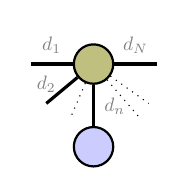
\begin{tikzpicture}[baseline=-0.5ex]
    \tikzset{tensor/.style = {minimum size = 0.5cm,shape = circle,thick,draw=black,inner sep = 0pt}, edge/.style = {thick,line width=.4mm},every loop/.style={}}
    \def\x{6}
    \node[tensor,fill=blue!20!white] (M) at (\x,-1.05) {$\vb$};
    \node[tensor,fill=green!50!red!50!white] (At) at 
    (\x,0) {$\Xt$};
    \draw[edge] (At) -- (\x-0.8,0) node [midway,above] {\scalebox{0.7}{\textcolor{gray}{$d_1$}}};
    \draw[edge] (At)-- (\x-0.6,-0.5) node [above]{\scalebox{0.7}{\textcolor{gray}{$d_2$}}};
    \draw[edge] (At) -- (\x+0.8,0) node [midway,above] {\scalebox{0.7}{\textcolor{gray}{$d_N$}}};;
    \draw[dotted] (At) -- (\x-0.3,-0.7);
    \draw[edge] (At) -- (\x,-0.8) node [midway,right] {\scalebox{0.7}{\textcolor{gray}{$d_n$}}};
    \draw[dotted] (At) -- (\x+0.6,-0.7);
    \draw[dotted] (At) -- (\x+0.7,-0.5);
    \end{tikzpicture}
\in\RR^{d_1\times  \dots\times d_{n-1}\times d_{n+1}\times \dots\times d_N}.
$$
注意，与模 $n$ 矩阵乘法不同，模 $n$ 向量乘法的相乘顺序会影响结果：向量收缩把张量的阶减 1，其后的模指标随之平移。设 $\Xt\in\RR^{d_1\times\cdots\times d_m\times\cdots\times d_n\times\cdots\times d_N}$ 且 $\ab\in\RR^{d_n},\bb\in\RR^{d_m}$，则
$
\Xt\ttm n \ab\ttm m\bb \neq
(\Xt \ttm m \bb)\ttm{n}\ab,
$
因为模 $n$ 向量乘法会去掉第 $m$ 维~\citep{bader2006algorithm}。
\end{enumerate}







下面介绍张量推导中常用的几种乘积：Kronecker 积、Khatri-Rao 积与 Hadamard 积。

\paragraph{Kronecker 积}\label{subsection-kron}
设 $\Ab\in\RR^{m\times n}$、$\Bb\in\RR^{p\times q}$。Kronecker 积 $\Ab\kron\Bb\in\RR^{mp\times nq}$ 定义为
\begin{align}
    \Ab\kron\Bb = 
    \begin{bmatrix}
    a_{11}\Bb & a_{12}\Bb & \dots & a_{1n}\Bb \\
    a_{21}\Bb & a_{22}\Bb & \dots & a_{2n}\Bb \\
    \vdots & \vdots & \ddots & \vdots \\
    a_{m1}\Bb & a_{m2}\Bb & \dots & a_{mn}\Bb 
    \end{bmatrix}.
\end{align}

在张量网络中，Kronecker 积由下图给出：
\begin{align}
    \Ab\kron\Bb = 
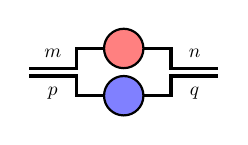
\begin{tikzpicture}[baseline=-0.5ex]
    \tikzset{tensor/.style = {minimum size = 0.5cm,shape = circle,thick,draw=black,inner sep = 0pt}, edge/.style   = {thick,line width=.4mm}}
    \def\x{0}
    \def\y{0}
    \node[tensor,fill=red!50!white] (A) at (\x,\y+0.3){$\Ab$};
    \node[tensor,fill=blue!50!white] (B) at (\x,\y-0.3){$\Bb$};
    \draw[edge] (\x-0.25,\y+0.3) -- (\x-0.6,\y+0.3) -- (\x-0.6,\y+0.05)   -- (\x-1.2,\y+0.05) node [midway,above] {\scalebox{0.7}{\dimcolor{$m$}}};
    \draw[edge] (\x-0.25,\y-0.3) -- (\x-0.6,\y-0.3) -- (\x-0.6,\y-0.05) -- (\x-1.2,\y-0.05) node [midway,below] {\scalebox{0.7}{\dimcolor{$p$}}};
    \draw[edge] (\x+0.25,\y+0.3) -- (\x+0.6,\y+0.3) -- (\x+0.6,\y+0.05) -- (\x+1.2,\y+0.05) node [midway,above] {\scalebox{0.7}{\dimcolor{$n$}}};
    \draw[edge] (\x+0.25,\y-0.3) -- (\x+0.6,\y-0.3) -- (\x+0.6,\y-0.05) -- (\x+1.2,\y-0.05) node [midway,below] {\scalebox{0.7}{\dimcolor{$q$}}};
\end{tikzpicture}.
\end{align}
从这张图可以看出，两个矩阵的 Kronecker 积不过是它们外积的一次重排。事实上，容易验证外积 $\Ab \outprod \Bb$ 的每个分量 $a_{i,j}b_{k,l}$ 都出现在 $\Ab \kron \Bb$ 中；外积是四阶张量，而 Kronecker 积是它的一种矩阵化。更精确地，可以证明 $\Ab \kron \Bb = (\Ab \outprod \Bb)_{(\{1,3\})}$，但我们不在此展开，而是相信张量网络图给出的简洁直观的看法：把 $\Ab$ 与 $\Bb$ 的行腿归到一侧、列腿归到另一侧，所得的矩阵就称为 $\Ab$ 与 $\Bb$ 的 Kronecker 积：
$$\Ab\outprod \Bb =    
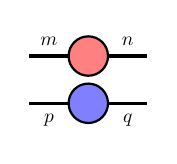
\begin{tikzpicture}[baseline=-0.5ex]
    \tikzset{tensor/.style = {minimum size = 0.5cm,shape = circle,thick,draw=black,inner sep = 0pt}, edge/.style   = {thick,line width=.4mm}}
    \def\x{0}
    \def\y{0}
    \node[tensor,fill=red!50!white] (A) at (\x,\y+0.3){$\Ab$};
    \node[tensor,fill=blue!50!white] (B) at (\x,\y-0.3){$\Bb$};
    \draw[edge] (\x-0.25,\y+0.3) -- (\x-0.75,\y+0.3) node [midway,above] {\scalebox{0.7}{\dimcolor{$m$}}};
    \draw[edge] (\x-0.25,\y-0.3) -- (\x-0.75,\y-0.3) node [midway,below] {\scalebox{0.7}{\dimcolor{$p$}}};
    \draw[edge] (\x+0.25,\y+0.3) -- (\x+0.75,\y+0.3) node [midway,above] {\scalebox{0.7}{\dimcolor{$n$}}};
    \draw[edge] (\x+0.25,\y-0.3) -- (\x+0.75,\y-0.3) node [midway,below] {\scalebox{0.7}{\dimcolor{$q$}}};
\end{tikzpicture}
\longrightarrow
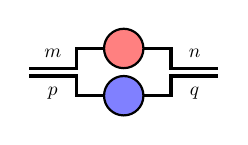
\begin{tikzpicture}[baseline=-0.5ex]
    \tikzset{tensor/.style = {minimum size = 0.5cm,shape = circle,thick,draw=black,inner sep = 0pt}, edge/.style   = {thick,line width=.4mm}}
    \def\x{0}
    \def\y{0}
    \node[tensor,fill=red!50!white] (A) at (\x,\y+0.3){$\Ab$};
    \node[tensor,fill=blue!50!white] (B) at (\x,\y-0.3){$\Bb$};
    \draw[edge] (\x-0.25,\y+0.3) -- (\x-0.6,\y+0.3) -- (\x-0.6,\y+0.05)   -- (\x-1.2,\y+0.05) node [midway,above] {\scalebox{0.7}{\dimcolor{$m$}}};
    \draw[edge] (\x-0.25,\y-0.3) -- (\x-0.6,\y-0.3) -- (\x-0.6,\y-0.05) -- (\x-1.2,\y-0.05) node [midway,below] {\scalebox{0.7}{\dimcolor{$p$}}};
    \draw[edge] (\x+0.25,\y+0.3) -- (\x+0.6,\y+0.3) -- (\x+0.6,\y+0.05) -- (\x+1.2,\y+0.05) node [midway,above] {\scalebox{0.7}{\dimcolor{$n$}}};
    \draw[edge] (\x+0.25,\y-0.3) -- (\x+0.6,\y-0.3) -- (\x+0.6,\y-0.05) -- (\x+1.2,\y-0.05) node [midway,below] {\scalebox{0.7}{\dimcolor{$q$}}};
\end{tikzpicture}
=\Ab \kron \Bb.
$$




更一般地，Kronecker 积可以定义在任意两个同阶张量之间。其做法是把两个张量的每一对腿
按次序两两归并到一起，例如，
$$
\At\kron\Bt = 
   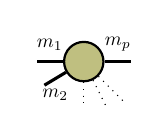
\begin{tikzpicture}[baseline=-0.5ex]
    \tikzset{tensor/.style = {minimum size = 0.5cm,shape = circle,thick,draw=black,inner sep = 0pt}, edge/.style = {thick,line width=.4mm},every loop/.style={}}
    \def\x{6}
    \node[tensor,fill=green!50!red!50!white] (A) at (\x,0) {$\At$};
    \draw[edge] (A) -- (\x-0.6,0) node [midway,above] {\scalebox{0.7}{\dimcolor{$m_1$}}};
    \draw[edge] (A) -- (\x+0.6,0) node [midway,above] {\scalebox{0.7}{\dimcolor{$m_p$}}};;
    \draw[edge] (A) -- (\x-0.5,-0.3) node [midway, below] {\scalebox{0.7}{\dimcolor{$m_2$}}};;
    \draw[dotted] (A) -- (\x,-0.6);
    \draw[dotted] (A) -- (\x,-0.6);
    \draw[dotted] (A) -- (\x+0.5,-0.5);

    \draw[dotted] (A) -- (\x+0.3,-0.6);
    \end{tikzpicture}
\kron
    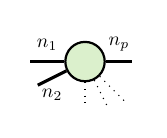
\begin{tikzpicture}[baseline=-0.5ex]
    \tikzset{tensor/.style = {minimum size = 0.5cm,shape = circle,thick,draw=black,inner sep = 0pt}, edge/.style = {thick,line width=.4mm},every loop/.style={}}
    \def\x{6}
    \def\y{0}
    \node[tensor,fill=green!70!red!20!white] (B) at (\x+1,\y) {$\Bt$};
    \draw[edge] (B) -- (\x+0.3,0) node [midway,above] {\scalebox{0.7}{\dimcolor{$n_1$}}};
    \draw[edge] (B) -- (\x+1.6,0) node [midway,above] {\scalebox{0.7}{\dimcolor{$n_p$}}};;
    \draw[edge] (B) -- (\x+0.4,-0.3) node [midway, below] {\scalebox{0.7}{\dimcolor{$n_2$}}};;
    \draw[dotted] (B) -- (\x+1,-0.6);
    \draw[dotted] (B) -- (\x+1.5,-0.5);
    \draw[dotted] (B) -- (\x+1.3,-0.6);
\end{tikzpicture}
=
    \begin{tikzpicture}[baseline=-0.5ex]
    \tikzset{tensor/.style = {minimum width = 3cm,minimum height = 0.6cm,shape = rounded rectangle,thick,draw=black,inner sep = 0pt}, edge/.style = {thick,line width=.4mm},every loop/.style={}}
    \def\x{0}
    \def\y{0}
    \node[tensor,fill=green!30!white] (At) at (\x,\y){$\At\kron\Bt$};
    \draw[edge] (\x-1.25,\y-0.3) -- (\x-1.25,\y-0.6) -- (\x-1.1,\y-0.6) -- (\x-1.1,\y-0.8);
    \draw[edge] (\x-0.85,\y-0.3) -- (\x-0.85,\y-0.6) -- (\x-1,\y-0.6) -- (\x-1,\y-0.8)node [below] {\scalebox{0.7}{\dimcolor{$m_1n_1$}}};
    \draw[edge] (\x-0.65,\y-0.3) -- (\x-0.65,\y-0.6) -- (\x-0.5,\y-0.6) -- (\x-0.5,\y-0.8);
    \draw[edge] (\x-0.25,\y-0.3) -- (\x-0.25,\y-0.6) -- (\x-0.4,\y-0.6) -- (\x-0.4,\y-0.8) node [below] {\scalebox{0.7}{\dimcolor{$m_2n_2$}}};
    \draw[edge] (\x+1.25,\y-0.3) -- (\x+1.25,\y-0.6) -- (\x+1.1,\y-0.6) -- (\x+1.1,\y-0.8);
    \draw[edge] (\x+0.85,\y-0.3) -- (\x+0.85,\y-0.6) -- (\x+1,\y-0.6) -- (\x+1,\y-0.8)  node [below] {\scalebox{0.7}{\dimcolor{$m_pn_p$}}};
    \draw[dotted] (\x+0.1,\y-0.3) -- (\x+0.1,\y-0.6) -- (\x+0.25,\y-0.6) -- (\x+0.25,\y-0.8);
    \draw[dotted] (\x+0.5,\y-0.3) -- (\x+0.5,\y-0.6) -- (\x+0.35,\y-0.6) -- (\x+0.35,\y-0.82) node [below] {\scalebox{0.7}{\dimcolor{$\dots$}}};;
    \end{tikzpicture}
    \in\RR^{m_1n_1\times\dots\times m_pn_p}.
$$

\begin{remark}
下面列出 Kronecker 积的一些有用性质。
\begin{enumerate}
    \item Kronecker 积不满足交换律，即一般地有 $\Ab\kron\Bb \neq \Bb\kron\Ab$%
    . 
    \item
    $
    \Ib\kron\Ab = 
    \begin{bmatrix}
    \Ab & 0 & \dots & 0\\
    0 & \Ab & \dots & 0\\
    \vdots & \vdots & \ddots & \vdots\\
    0 & 0 & \dots & \Ab
    \end{bmatrix}
    $
    是分块对角矩阵。
    \item 两个同阶张量的 Kronecker 积仍是同阶张量，而它们的外积则使阶数翻倍。
    \item 
    对 Kronecker 积 $\Ab\kron\Bb$ 作重排，即可得到外积 $\Ab\outprod\Bb$。
 \item
两个{单位矩阵}的 Kronecker 积是更大的单位矩阵，即 $\Ib_m \kron \Ib_n = \Ib_{mn}$，画出张量网络图便不难看出：
$$
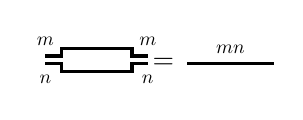
\begin{tikzpicture}[baseline=-0.5ex]
    \tikzset{tensor/.style = {minimum width = 3cm,minimum height = 0.6cm,shape = rounded rectangle,thick,draw=black,inner sep = 0pt}, edge/.style = {thick,line width=.4mm},every loop/.style={}}
    \def\x{0}
    \def\y{0.1}
    \draw[edge](\x-0.1,\y) node [above] {\scalebox{0.7}{\dimcolor{$m$}}}  -- (\x+0.1,\y) -- (\x+0.1,\y+0.1)--(\x+1,\y+0.1) -- (\x+1,\y)-- (\x+1.2,\y) node [above] {\scalebox{0.7}{\dimcolor{$m$}}};
    \draw[edge](\x-0.1,\y-0.1)  node [below] {\scalebox{0.7}{\dimcolor{$n$}}}  -- (\x+0.1,\y-0.1) -- (\x+0.1,\y-0.2)--(\x+1,\y-0.2) -- (\x+1,\y-0.1) --(\x+1.2,\y-0.1)  node [below] {\scalebox{0.7}{\dimcolor{$n$}}} ;
    \node[draw=none] at (\x+1.4,\y-0.1) {\scalebox{1}{\textcolor{black}{$=$}}};
    \draw[edge](\x+1.7,\y-0.1) -- (\x+2.8,\y-0.1) node [midway, above] {\scalebox{0.7}{\dimcolor{$mn$}}} ;
\end{tikzpicture}.
$$
     \item
     两个向量的 Kronecker 积就是它们外积的向量化：
     $$\vectorize(\ub \outprod \vb) = \vectorize(\ub  \vb^\ts) =\ub \kron \vb =  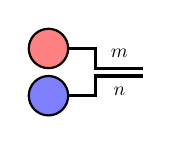
\begin{tikzpicture}[baseline=-0.5ex]
    \tikzset{tensor/.style = {minimum size = 0.5cm,shape = circle,thick,draw=black,inner sep = 0pt}, edge/.style   = {thick,line width=.4mm}}
    \def\x{0}
    \def\y{0}
    \node[tensor,fill=red!50!white] (A) at (\x,\y+0.3){$\ub$};
    \node[tensor,fill=blue!50!white] (B) at (\x,\y-0.3){$\vb$};
    \draw[edge] (\x+0.25,\y+0.3) -- (\x+0.6,\y+0.3) -- (\x+0.6,\y+0.05) -- (\x+1.2,\y+0.05) node [midway,above] {\scalebox{0.7}{\dimcolor{$m$}}};
    \draw[edge] (\x+0.25,\y-0.3) -- (\x+0.6,\y-0.3) -- (\x+0.6,\y-0.05) -- (\x+1.2,\y-0.05) node [midway,below] {\scalebox{0.7}{\dimcolor{$n$}}};
\end{tikzpicture}
    .$$
    \item 
   Kronecker 积满足所谓的\textit{混合乘积}性质：$(\Ab\kron \Bb)(\Cb\kron\Db) = \Ab\Cb\kron\Bb\Db$，其中 $\Ab\in\RR^{m\times n},\Bb\in\RR^{p\times q},\Cb\in\RR^{n\times d}$、$\Db\in\RR^{q\times k}$。
\begin{proof}
 \begin{align*}
(\Ab\kron\Bb)(\Cb\kron\Db) 
&= 
\begin{tikzpicture}[baseline=\baseline]
    \tikzset{tensor/.style = {minimum size = 0.5cm,shape = circle,thick,draw=black,inner sep = 0pt}, edge/.style   = {thick,line width=.4mm}}
    \def\y{0.4}\def\x{0}
    \draw[edge] (\x-1,\y-0.3) -- (\x-0.7,\y-0.3) -- (\x-0.7,\y+0.1)   -- (\x+0.7,\y+0.1) -- (\x+0.7,\y-0.3) -- (\x+1.1,\y-0.3);
    \node[tensor,fill=red!50!white] (A) at (\x,\y){$\Ab$};
    \draw[edge] (\x+1,\y-0.3) -- (\x+1.3,\y-0.3) -- (\x+1.3,\y+0.1)   -- (\x+2.6,\y+0.1) -- (\x+2.6,\y-0.3) -- (\x+3,\y-0.3);
    \node[tensor,fill=orange!50!white] (C) at (\x+2,\y){$\Cb$};
    \def\y{-0.4}\def\x{0}
    \draw[edge] (\x-1,\y+0.4) -- (\x-0.7,\y+0.4) -- (\x-0.7,\y+0.1) -- (\x+0.7,\y+0.1) -- (\x+0.7,\y+0.4) -- (\x+0.7,\y+0.4) -- (\x+1.1,\y+0.4);
    \node[tensor,fill=blue!50!white] (B) at (\x,\y+0.1){$\Bb$};
    \draw[edge] (\x+1,\y+0.4) -- (\x+1.3,\y+0.4) -- (\x+1.3,\y+0.1) -- (\x+2.6,\y+0.1) -- (\x+2.6,\y+0.4) -- (\x+2.6,\y+0.4) -- (\x+3,\y+0.4);
    \node[draw=none] () at (\x+3.25,\y+0.45) {\scalebox{0.7}{\dimcolor{$dk$}}};
    \node[tensor,fill=green!50!red!40!white] (D) at (\x+2,\y+0.1){$\Db$};
    \node[draw=none] () at (\x+1,\y+0.7) {\scalebox{0.7}{\dimcolor{$nq$}}};
    \node[draw=none] () at (\x-1.25,\y+0.4) {\scalebox{0.7}{\dimcolor{$mp$}}};
\end{tikzpicture}\\
 &=
 \begin{tikzpicture}[baseline=\baseline]
    \tikzset{tensor/.style = {minimum size = 0.5cm,shape = circle,thick,draw=black,inner sep = 0pt}, edge/.style   = {thick,line width=.4mm}}
    \def\y{0.4}\def\x{0}
    \draw[edge] (\x-1,\y-0.35) -- (\x-0.7,\y-0.35) -- (\x-0.7,\y)   -- (\x,\y) -- (\x+0.5,\y) -- (\x+0.8,\y);
    \node[tensor,fill=red!50!white] (A) at (\x,\y){$\Ab$};
    \draw[edge] (\x+1.2,\y) -- (\x+1.7,\y) -- (\x+1.7,\y-0.35) -- (\x+2.1,\y-0.35);
    \node[tensor,fill=orange!50!white] (C) at (\x+1,\y){$\Cb$};
    \def\y{-0.4}\def\x{0}
    \draw[edge] (\x-1,\y+0.35) -- (\x-0.7,\y+0.35) -- (\x-0.7,\y) -- (\x,\y) -- (\x+0.8,\y);
    \node[tensor,fill=blue!50!white] (B) at (\x,\y){$\Bb$};
    \draw[edge] (\x+1,\y) -- (\x+1.7,\y) -- (\x+1.7,\y+0.35) -- (\x+2.1,\y+0.35);
    \node[draw=none] () at (\x+2.35,\y+0.4) {\scalebox{0.7}{\dimcolor{$dk$}}};
    \node[tensor,fill=green!50!red!40!white] (D) at (\x+1,\y){$\Db$};
    \node[draw=none] () at (\x-1.25,\y+0.35) {\scalebox{0.7}{\dimcolor{$mp$}}};
    \node[draw=none] () at (\x+0.5,\y+1) {\scalebox{0.7}{\dimcolor{$n$}}};
     \node[draw=none] () at (\x+0.5,\y+0.2) {\scalebox{0.7}{\dimcolor{$q$}}};
\end{tikzpicture}\\
&=
\Ab\Cb\kron\Bb\Db.
    \end{align*}
\end{proof}
特别地，$(\Ab\kron\Ib)(\Ib\kron\Bb)=\Ab\kron\Bb$。 
\item 由上面的推导可以看出，在处理含 Kronecker 积的恒等式时，常常需要把
$
    \begin{tikzpicture}[baseline=\baseline]
    \tikzset{tensor/.style = {minimum size = 0.5cm,shape = circle,thick,draw=black,inner sep = 0pt}, edge/.style   = {thick,line width=.4mm}}
    \def\y{0.6}\def\x{0}
    \draw[edge] (\x+3,\y-0.3)  node [above] {\scalebox{0.7}{\textcolor{gray}{$p$}}} -- (\x+4,\y-0.3)node [above] {\scalebox{0.7}{\textcolor{gray}{$n$}}};
    \def\y{-0.6}\def\x{0}
    \draw[edge] (\x+3,\y+0.3) node [above] {\scalebox{0.7}{\dimcolor{$m$}}}-- (\x+4,\y+0.3)node [above] {\scalebox{0.7}{\dimcolor{$q$}}};
    \end{tikzpicture}
$
重排成
$
 \begin{tikzpicture}[baseline=\baseline]
    \tikzset{tensor/.style = {minimum size = 0.5cm,shape = circle,thick,draw=black,inner sep = 0pt}, edge/.style   = {thick,line width=.4mm}}
    \def\y{0.4}\def\x{0}
    \draw[edge] (\x-1,\y-0.3) -- (\x-0.7,\y-0.3)-- (\x-0.7,\y+0.1) -- (\x+0.7,\y+0.1) -- (\x+0.7,\y-0.3) -- (\x+1.1,\y-0.3);
    \node[draw=none] () at (\x+1.35,\y-0.4) {\scalebox{0.7}{\dimcolor{$nq$}}};
    \node[draw=none] () at (\x-1.25,\y-0.4) {\scalebox{0.7}{\dimcolor{$pm$}}};
    \def\y{-0.4}\def\x{0}
    \draw[edge] (\x-1,\y+0.4) -- (\x-0.7,\y+0.4) -- (\x-0.7,\y+0.1) -- (\x+0.7,\y+0.1) -- (\x+0.7,\y+0.4) -- (\x+0.7,\y+0.4) -- (\x+1.1,\y+0.4);
    \end{tikzpicture}
$，反之亦然。
\item 对 $\Ab\in\RR^{m\times m}$ 与 $\Bb\in\RR^{n\times n},$，有等式 $\tr(\Ab\kron\Bb)=\tr(\Ab)\tr(\Bb)$，由下图不难证明：
$$
\tr(\Ab\kron\Bb) = 
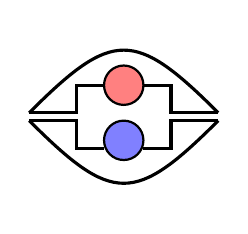
\begin{tikzpicture}[baseline=-0.5ex]
    \tikzset{tensor/.style = {minimum size = 0.5cm,shape = circle,thick,draw=black,inner sep = 0pt}, edge/.style   = {thick,line width=.4mm}}
    \def\x{0}
    \def\y{0}
    \node[tensor,fill=red!50!white] (A) at (\x,\y+0.5){$\Ab$};
    \node[tensor,fill=blue!50!white] (B) at (\x,\y-0.2){$\Bb$};
    \draw[edge] (\x-0.25,\y+0.5) -- (\x-0.6,\y+0.5) -- (\x-0.6,\y+0.15)   -- (\x-1.2,\y+0.15);
    \draw[edge] (\x-0.25,\y-0.3) -- (\x-0.6,\y-0.3) -- (\x-0.6,\y+0.05) -- (\x-1.2,\y+0.05);
    \draw[edge] (\x+0.25,\y+0.5) -- (\x+0.6,\y+0.5) -- (\x+0.6,\y+0.15) -- (\x+1.2,\y+0.15);
    \draw[edge] (\x+0.25,\y-0.3) -- (\x+0.6,\y-0.3) -- (\x+0.6,\y+0.05) -- (\x+1.2,\y+0.05);
    \draw[edge](\x-1.2,\y+0.15) to [out=45,in=135, distance=1.5cm] (\x+1.2,\y+0.15);
    \draw[edge](\x-1.2,\y+0.05) to [out=-45,in=-135, distance=1.5cm] (\x+1.2,\y+0.05);
\end{tikzpicture}
=
\tr(\Ab)\tr(\Bb).
$$

\item \textbf{Sylvester 恒等式（Sylvester identity）}是一条联系向量化、矩阵乘法与 Kronecker 积的非常有用的恒等式：$$\vectorize(\Ab\Xb\Bb) = (\Ab\kron \Bb^\ts)\vectorize(\Xb),$$
其中 $\Ab\in\RR^{m\times n},\Xb\in\RR^{n\times p}$ 且 $\Bb\in\RR^{p\times q}.$
\begin{proof}
利用张量网络，证明相当直接： 
\begin{align*}
\vectorize(\Ab\Xb\Bb) &=
 \vectorize\left(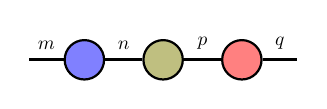
\begin{tikzpicture}[baseline=-0.5ex]
    \tikzset{tensor/.style = {minimum size = 0.5cm,shape = circle,thick,draw=black,inner sep = 0pt}, edge/.style = {thick,line width=.4mm},every loop/.style={}}
    \def\x{6}
    \node[tensor,fill=blue!50!white] (A) at (\x-1,0) {$\Ab$};
    \node[tensor,fill=green!50!red!50!white] (X) at (\x,0) {$\Xb$};
    \node[tensor,fill=red!50!white] (B) at (\x+1,0) {$\Bb$};
    \draw[edge] (A) -- (X) node [midway,above] {\scalebox{0.7}{\dimcolor{$n$}}};
    \draw[edge] (X) -- (B) node [midway,above] {\scalebox{0.7}{\dimcolor{$p$}}};
    \draw[edge] (A) -- (\x-1.7,0) node [midway,above] {\scalebox{0.7}{\dimcolor{$m$}}};
    \draw[edge] (B) -- (\x+1.7,0) node [midway,above] {\scalebox{0.7}{\dimcolor{$q$}}};
    \end{tikzpicture}\right)
=
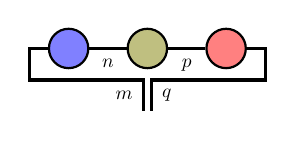
\begin{tikzpicture}[baseline=-0.5ex]
    \tikzset{tensor/.style = {minimum size = 0.5cm,shape = circle,thick,draw=black,inner sep = 0pt}, edge/.style = {thick,line width=.4mm},every loop/.style={}}
    \def\x{6}
    \node[tensor,fill=blue!50!white] (A) at (\x-1,0) {$\Ab$};
    \node[tensor,fill=green!50!red!50!white] (X) at (\x,0) {$\Xb$};
    \node[tensor,fill=red!50!white] (B) at (\x+1,0) {$\Bb$};
    \draw[edge] (A) -- (X) node [midway,below] {\scalebox{0.7}{\dimcolor{$n$}}};
    \draw[edge] (X) -- (B) node [midway,below] {\scalebox{0.7}{\dimcolor{$p$}}};
    \draw[edge] (A) -- (\x-1.5,0) -- (\x-1.5,-0.4) -- (\x-0.05,-0.4)--(\x-0.05,-0.8) node [midway,left] {\scalebox{0.7}{\dimcolor{$m$}}};
    \draw[edge] (B) -- (\x+1.5,0) -- (\x+1.5,-0.4) -- (\x+0.05,-0.4)--(\x+0.05,-0.8) node [midway,right] {\scalebox{0.7}{\dimcolor{$q$}}};
\end{tikzpicture}\\
&=
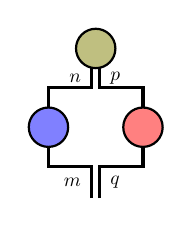
\begin{tikzpicture}[baseline=-2ex]
    \tikzset{tensor/.style = {minimum size = 0.5cm,shape = circle,thick,draw=black,inner sep = 0pt}, edge/.style = {thick,line width=.4mm},every loop/.style={}}
    \def\x{6}
    \draw[edge] (\x-0.05,0.25) -- (\x-0.05,0) node [midway, left] {\scalebox{0.7}{\dimcolor{$n$}}}   -- (\x-0.6,0) -- (\x-0.6,-0.25) ; 
    \draw[edge] (\x+0.05,0.25) -- (\x+0.05,0)   node [midway, right] {\scalebox{0.7}{\dimcolor{$p$}}}  -- (\x+0.6,0) -- (\x+0.6,-0.25);    
    \draw[edge] (\x-0.05,-1.4) -- (\x-0.05,-1)  node [midway, left] {\scalebox{0.7}{\dimcolor{$m$}}}  -- (\x-0.6,-1) -- (\x-0.6,-0.75) ; 
    \draw[edge] (\x+0.05,-1.4) -- (\x+0.05,-1)  node [midway, right] {\scalebox{0.7}{\dimcolor{$q$}}}   -- (\x+0.6,-1) -- (\x+0.6,-0.75); 
     \node[tensor,fill=green!50!red!50!white] (X) at (\x,0.5) {$\Xb$};
    \node[tensor,fill=blue!50!white] (A) at (\x-0.6,-0.5) {$\Ab$};
    \node[tensor,fill=red!50!white] (B) at (\x+0.6,-0.5) {$\Bb$};
\end{tikzpicture}
=
(\Ab\kron\Bb^\ts)\vectorize(\Xb).
\end{align*}
在最后一个图中，容易看出 $\Xb$ 的向量化以及 $\Ab$ 与 $\Bb$ 的 Kronecker 积，从而可以断定该张量网络表示二者之间的矩阵-向量乘法。然而，把张量网络翻译成经典数学记法时需要注意一些细节。首先，由于 $\vectorize(\Xb)$ 的维度为 $np$，Kronecker 积必须取在 $\Ab$ 与 $\Bb^\ts$ 之间，才能得到形状为 $mq\times np$ 的矩阵。其次，需要确定使用哪一个 Kronecker 积：$\Ab \kron \Bb^\ts$ 还是 $\Bb^\ts \kron \Ab$，二者的形状都正确。由于本手稿对 $\vectorize$ 这类重排运算采用字典序，正确的写法是  $\Ab \kron \Bb^\ts$。然而，若采用逆字典序，如~\citep{kolda2009tensor} 中的做法，正确的写法应为 $\Bb^\ts \kron \Ab$。
\end{proof}
\emph{Sylvester 恒等式}是求解形如 $\Ab\Xb+\Xb\Bb = \Cb$ 的方程组的有用恒等式。
\end{enumerate}
\end{remark}
模 $n$ 乘积、矩阵化与 Kronecker 积之间存在若干有用的关系： 
\begin{proposition}
设 $\Tt\in\RR^{d_1\times d_2\times\dots\times d_p}$，$\Ab_1\in\RR^{d_1\times n_1},
\Ab_2\in\RR^{d_2\times n_2},\dots,$
$\Ab_p\in\RR^{d_p\times n_p}$，则 
\begin{align*}(\Tt\ttm1\Ab_1\ttm2\Ab_2\ttm3\Ab_3\ttm4\dots\ttm p\Ab_p)_{(n)}=
\Ab_n\Tt_{(n)}(\Ab_1\kron\dots\kron\Ab_{n-1}\kron\Ab_{n+1}\kron\dots\kron\Ab_p)^\ts.
\end{align*}
\end{proposition}
\begin{proof}
当 $p =3$ 且 $n=1$ 时，
\begin{align*}
(\Tt\ttm1\Ab_1\ttm2\Ab_2\ttm3\Ab_3)_{(1)}
&= 
 \left(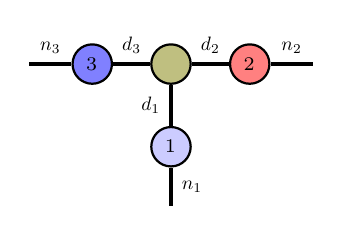
\begin{tikzpicture}[baseline=-0.5ex]
    \tikzset{tensor/.style = {minimum size = 0.5cm,shape = circle,thick,draw=black,inner sep = 0pt}, edge/.style = {thick,line width=.4mm},every loop/.style={}}
    \def\x{6}
    \node[tensor,fill=blue!20!white] (A1) at (\x,-1.05) {$\Ab_1$};
    \node[tensor,fill=green!50!red!50!white] (At) at (\x,0) {$\Tt$};
    \node[tensor,fill=red!50!white] (A2) at (\x+1,0) {$\Ab_2$};
    \node[tensor,fill=blue!50!white] (A3) at (\x-1,0) {$\Ab_3$};
    \draw[edge] (At) -- (A2) node [midway,above] {\scalebox{0.7}{\dimcolor{$d_2$}}};
    \draw[edge] (At) -- (A1) node [midway,left] {\scalebox{0.7}{\dimcolor{$d_1$}}};
    \draw[edge] (At) -- (A3) node [midway,above] {\scalebox{0.7}{\dimcolor{$d_3$}}};
    \draw[edge] (A1) -- (\x,-1.8) node [midway,right] {\scalebox{0.7}{\dimcolor{$n_1$}}};
    \draw[edge] (A2) -- (\x+1.8,0) node [midway,above] {\scalebox{0.7}{\dimcolor{$n_2$}}};
    \draw[edge] (A3) -- (\x-1.8,0) node [midway,above] {\scalebox{0.7}{\dimcolor{$n_3$}}};
    \end{tikzpicture}\right)_{(1)}
=
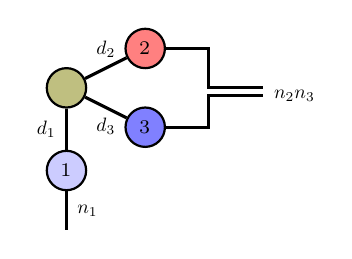
\begin{tikzpicture}[baseline=-0.5ex]
    \tikzset{tensor/.style = {minimum size = 0.5cm,shape = circle,thick,draw=black,inner sep = 0pt}, edge/.style = {thick,line width=.4mm},every loop/.style={}}
    \def\x{6}
    \def\y{0}
    \node[tensor,fill=blue!20!white] (A1) at (\x,-1.05) {$\Ab_1$};
    \node[tensor,fill=green!50!red!50!white] (At) at (\x,0) {$\Tt$};
    \node[tensor,fill=red!50!white] (A2) at (\x+1,\y+0.5) {$\Ab_2$};
    \node[tensor,fill=blue!50!white] (A3) at (\x+1,\y-0.5) {$\Ab_3$};
    \draw[edge] (At) -- (A1) node [midway,left] {\scalebox{0.7}{\dimcolor{$d_1$}}};
    \draw[edge] (At) -- (A3) node [midway,below] {\scalebox{0.7}{\dimcolor{$d_3$}}};
    \draw[edge] (At) -- (A2) node [midway,above] {\scalebox{0.7}{\dimcolor{$d_2$}}};
    \draw[edge] (A1) -- (\x,-1.8) node [midway,right] {\scalebox{0.7}{\dimcolor{$n_1$}}};
    \draw[edge] (A2) -- (\x+1.8,\y+0.5) -- (\x+1.8,\y)-- (\x+2.5,\y);
    \draw[edge] (A3) -- (\x+1.8,\y-0.5) -- (\x+1.8,\y-0.1) -- (\x+2.5,\y-0.1)node [right] {\scalebox{0.7}{\dimcolor{$n_2n_3$}}};
    \end{tikzpicture}\\
&=
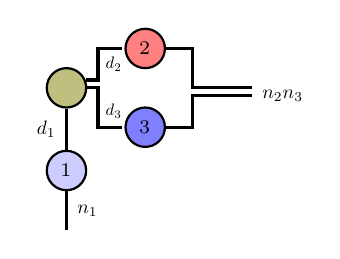
\begin{tikzpicture}[baseline=-0.5ex]
    \tikzset{tensor/.style = {minimum size = 0.5cm,shape = circle,thick,draw=black,inner sep = 0pt}, edge/.style = {thick,line width=.4mm},every loop/.style={}}
    \def\x{6}
    \def\y{0}
    \node[tensor,fill=blue!20!white] (A1) at (\x,-1.05) {$\Ab_1$};
    \node[tensor,fill=green!50!red!50!white] (At) at (\x,0) {$\Tt$};
    \node[tensor,fill=red!50!white] (A2) at (\x+1,\y+0.5) {$\Ab_2$};
    \node[tensor,fill=blue!50!white] (A3) at (\x+1,\y-0.5) {$\Ab_3$};
    \draw[edge] (At) -- (A1) node [midway,left] {\scalebox{0.7}{\dimcolor{$d_1$}}};
    \draw[edge] (\x+0.7,\y-0.5) -- (\x+0.4,\y-0.5) -- (\x+0.4,\y) -- (\x+0.25,\y);
    \draw[edge] (\x+0.7,\y+0.5) -- (\x+0.4,\y+0.5) -- (\x+0.4,\y+0.1) -- (\x+0.25,\y+0.1);
    \draw[edge] (A1) -- (\x,-1.8) node [midway,right] {\scalebox{0.7}{\dimcolor{$n_1$}}};
    \draw[edge] (A2) -- (\x+1.6,\y+0.5) -- (\x+1.6,\y)-- (\x+2.35,\y);
    \draw[edge] (A3) -- (\x+1.6,\y-0.5) -- (\x+1.6,\y-0.1) -- (\x+2.35,\y-0.1)node [right] {\scalebox{0.7}{\dimcolor{$n_2n_3$}}};
    \node[draw=none] () at (\x+0.6,\y-0.3) {\scalebox{0.6}{\dimcolor{$d_3$}}};
    \node[draw=none] () at (\x+0.6,\y+0.3) {\scalebox{0.6}{\dimcolor{$d_2$}}};
\end{tikzpicture}
=
\Ab_1\Tt_{(1)}(\Ab_2\kron\Ab_3)^\ts.
\end{align*}
\end{proof}
\begin{proposition}
    设 $\Tt\in\RR^{d_1\times d_2\times\cdots\times d_p}$  且对 $i\in[p]$ 有 $\Ab_i\in\RR^{d_i\times n_i}$。设 $m \in [p]$，
记 $\Tt_{([m])}$ 表示把张量 $\Tt$ 重排为尺寸 $d_1d_2\cdots d_m\times d_{m+1}...d_p$ 的矩阵：前 $m$ 个指标映射到
行，其余指标映射到列。于是，
\begin{align*}
    (\Tt\ttm 1\Ab_1\ttm 2 \Ab_2\cdots\ttm p \Ab_p)_{([m])}=(\Ab_1\kron\Ab_2\kron\cdots\kron\Ab_{m})\Tb_{([m])}(\Ab_{m+1}\kron\Ab_{m+2}\kron\cdots\kron\Ab_{p})^\ts.
\end{align*}
此恒等式可推广到任意子集 $I\subset [p]$：
$$ (\Tt\ttm 1\Ab_1\ttm 2 \Ab_2\cdots\ttm p \Ab_p)_{(I)}    = \left(\bigotimes_{i\in I} \Ab_i\right)\Tt_{([m])}\left(\bigotimes_{i\in [p] \setminus I} \Ab_i\right)^\ts.$$
\begin{proof}
当 $p=6$ 且 $I = \{1,2,3\}$ 时，
\begin{align*}
\left(\begin{tikzpicture}[baseline=\baseline]
    \tikzset{tensor/.style = {minimum size = 0.5cm,shape = circle,thick,draw=black,inner sep = 0pt}, edge/.style = {thick,line width=.4mm},every loop/.style={}}
    \def\y{0}
    \def\x{0}
    \node[tensor,fill=red!20!blue!40!white] (T) at (\x,\y){\scalebox{0.85}{$\Tt$}};
\node[tensor,fill=red!20!white] (A) at (\x+1,\y){\scalebox{0.85}{$\Ab_1$}};
    \draw[edge](T) -- (A) node [midway,above] {\scalebox{0.7}{\dimcolor{$d_1$}}};
    \draw[edge](A) -- (\x+2,\y) node [midway,above] {\scalebox{0.7}{\dimcolor{$n_1$}}};
\node[tensor,fill=red!40!white] (B) at (\x,\y-1) {\scalebox{0.85}{$\Ab_2$}}; 
    \draw[edge](T) -- (B) node [midway,left] {\scalebox{0.7}{\dimcolor{$d_2$}}};
    \draw[edge](B) -- (\x,\y-2) node [midway,left] {\scalebox{0.7}{\dimcolor{$n_2$}}};
\node[tensor,fill=red!60!white] (C) at (\x-1,\y) {\scalebox{0.85}{$\Ab_3$}};
    \draw[edge](T) -- (C) node [midway,above] {\scalebox{0.7}{\dimcolor{$d_3$}}};
    \draw[edge](C) -- (\x-2,\y) node [midway,above] {\scalebox{0.7}{\dimcolor{$n_3$}}};
\node[tensor,fill=blue!20!white] (D) at (\x,\y+1){\scalebox{0.85}{$\Ab_4$}}; 
    \draw[edge](T) -- (D) node [midway,right] {\scalebox{0.7}{\dimcolor{$d_4$}}};
    \draw[edge](D) -- (\x,\y+2) node [midway,right] {\scalebox{0.7}{\dimcolor{$n_4$}}};
\node[tensor,fill=red!50!blue!10!white] (E) at (\x-0.85,\y+0.85){\scalebox{0.85}{$\Ab_5$}}; 
   \draw[edge](T) -- (E) node [midway,above] {\scalebox{0.7}{\dimcolor{$d_5$}}};
    \draw[edge](E) -- (\x-1.5,\y+1.5) node [midway,right] {\scalebox{0.7}{\dimcolor{$n_5$}}};
\node[tensor,fill=blue!50!white] (F) at (\x+0.85,\y-0.85){\scalebox{0.85}{$\Ab_6$}};
    \draw[edge](T) -- (F)node [midway,right] {\scalebox{0.7}{\dimcolor{$d_6$}}};
    \draw[edge](F) -- (\x+1.5,\y-1.5)node [midway,right] {\scalebox{0.7}{\dimcolor{$n_6$}}};
\end{tikzpicture}\right)_{(\{1,2,3\})}
\begin{tikzpicture}[baseline=\baseline]
    \tikzset{tensor/.style = {minimum size = 0.5cm,shape = circle,thick,draw=black,inner sep = 0pt}, edge/.style = {thick,line width=.4mm},every loop/.style={}}
    \def\y{0}
    \def\x{0}
    \node[draw=none] at (\x-3.5,\y){$=$};
    \node[tensor,fill=red!20!blue!40!white] (T) at (\x,\y){\scalebox{0.85}{$\Tb$}};
    \node[tensor,fill=red!20!white] (A) at (\x-1.5,\y-1){\scalebox{0.85}{$\Ab_1$}};
    \node[tensor,fill=red!40!white] (B) at (\x-1.5,\y) {\scalebox{0.85}{$\Ab_2$}}; 
    \node[tensor,fill=red!60!white] (C) at (\x-1.5,\y+1) {\scalebox{0.85}{$\Ab_3$}};
    \node[tensor,fill=blue!20!white] (D) at (\x+1.5,\y-1){\scalebox{0.85}{$\Ab_4$}};
\node[tensor,fill=red!50!blue!10!white] (E) at (\x+1.5,\y){\scalebox{0.85}{$\Ab_5$}}; 
\node[tensor,fill=blue!50!white] (F) at (\x+1.5,\y+1){\scalebox{0.85}{$\Ab_6$}};
    \draw[edge](T) -- (B);
    \node[draw=none] at (\x-1.15,\y+0.2) {\scalebox{0.7}{\dimcolor{$d_2$}}};;
    \node[draw=none] at (\x+1.15,\y+0.2) {\scalebox{0.7}{\dimcolor{$d_5$}}};;
    \draw[edge](B) -- (\x-2.5,\y);;
    \draw[edge](\x+0.16,\y+0.2) -- (\x+0.5,\y+0.2) -- (\x+0.5,\y+0.1) -- (\x+1,\y+0.1);
    \draw[edge](F) -- (\x+1,\y+1) -- (\x+1,\y+0.1)node [midway,left] {\scalebox{0.7}{\dimcolor{$d_6$}}};
    \draw[edge](F) -- (\x+2,\y+1)--(\x+2,\y+0.1)-- (\x+2.5,\y+0.1)node [near end,above] {\scalebox{0.7}{\dimcolor{$n_6$}}};
    \draw[edge](\x+0.16,\y-0.2) -- (\x+0.5,\y-0.2) -- (\x+0.5,\y-0.1) -- (\x+1,\y-0.1);
    \draw[edge](D) -- (\x+1,\y-1) -- (\x+1,\y-0.1)node [midway,left] {\scalebox{0.7}{\dimcolor{$d_4$}}};
    \draw[edge](D) -- (\x+2,\y-1)--(\x+2,\y-0.1)-- (\x+2.5,\y-0.1)node [near end,below] {\scalebox{0.7}{\dimcolor{$n_4$}}};
    \draw[edge](T) -- (E);
    \draw[edge](E) -- (\x+2.5,\y);
    \draw[edge](\x-0.16,\y+0.2) -- (\x-0.5,\y+0.2) -- (\x-0.5,\y+0.1) -- (\x-1,\y+0.1);
    \draw[edge](C) -- (\x-1,\y+1) -- (\x-1,\y+0.1)node [midway,right] {\scalebox{0.7}{\dimcolor{$d_3$}}};
    \draw[edge](C) -- (\x-2,\y+1)--(\x-2,\y+0.1)-- (\x-2.5,\y+0.1)node [near end,above] {\scalebox{0.7}{\dimcolor{$n_3$}}};;;
    \draw[edge](\x-0.16,\y-0.2) -- (\x-0.5,\y-0.2) -- (\x-0.5,\y-0.1) -- (\x-1,\y-0.1);
    \draw[edge](A) --  (\x-2,\y-1)--(\x-2,\y-0.1)-- (\x-2.5,\y-0.1)node [near end,below] {\scalebox{0.7}{\dimcolor{$n_1$}}};;
    \draw[edge](A) -- (\x-1,\y-1) -- (\x-1,\y-0.1)node [midway,right] {\scalebox{0.7}{\dimcolor{$d_1$}}};
    \node[draw=none] at (\x+2.8,\y){\scalebox{0.7}{\dimcolor{$n_4$}}};
    \node[draw=none] at (\x-2.8,\y){\scalebox{0.7}{\dimcolor{$n_2$}}};
\end{tikzpicture}.
\end{align*}
\end{proof}
\end{proposition}


\paragraph{Khatri-Rao 积}
Khatri-Rao 积是按列进行的 Kronecker 积~\citep{smilde2005multi,bro1998multi}。设 $\Ab\in\RR^{m\times R}$ 且 $\Bb\in\RR^{n\times R}$。$\Ab$ 与 $\Bb$ 的 Khatri-Rao 积记为 $\Ab\krao\Bb\in\RR^{mn\times R}$，定义为
\begin{align*}
    \def\baseline{-0.5ex}
    \Ab\krao\Bb =
    \begin{bmatrix}
    \vline & \vline  &   & \vline \\
    \ab_1\kron\bb_1 & \ab_2\kron\bb_2 & \dots & \ab_R\kron\bb_R\\
    \vline & \vline & & \vline 
    \end{bmatrix}
=
    \begin{tikzpicture}[baseline=\baseline]
    \tikzset{tensor/.style = {minimum size = 0.5cm,shape = circle,thick,draw=black,inner sep = 0pt}, edge/.style   = {thick,line width=.4mm},every loop/.style={}}
    \def\y{0}
    \def\x{0}
    \node[tensor,fill=red!50!white] (A) at (\x,\y){$\Ab$};
    \node[tensor,fill=blue!50!white] (B) at (\x+1,\y){$\Bb$};
    \draw[edge] (\x,\y+0.25) -- (\x,\y+0.5) -- (\x+0.5,\y+0.7);
    \draw[edge] (\x+1,\y+0.25) -- (\x+1,\y+0.5) -- (\x+0.5,\y+0.7);
    \draw[edge] (\x+0.5,\y+0.7) -- (\x+0.5,\y+1.2) node [left, midway] {\edgelabel{$R$}};
    \draw  node[fill = black,circle,inner sep=0pt,minimum size=4pt] (m) at (\x+0.5,\y+0.7) {};
    \draw[edge] (\x,\y-0.25) -- (\x,\y-0.7);
    \draw[edge] (\x+1,\y-0.25) -- (\x+1,\y-0.7);
    \draw[edge] (\x+1,\y-0.7) -- (\x+0.5,\y-0.7) -- (\x+0.5,\y-1);
    \draw[edge] (\x+1,\y-0.25) -- (\x+1,\y-0.7);
    \draw[edge] (\x,\y-0.7) -- (\x+0.4,\y-0.7) -- (\x+0.4,\y-1)node [below] {\edgelabel{$mn$}};
    \end{tikzpicture}\hspace{0.5cm},
\end{align*}
其中 $\ab_1,\dots,\ab_R\in\RR^{m}$ 为 $\Ab$ 的各列，$\bb_1,\dots,\bb_R\in\RR^{n}$ 为 $\Bb$ 的各列。  在对应的张量网络图中，复制张量强制所得矩阵只包含 $\Ab$ 与 $\Bb$ 中\emph{相互匹配}的各列的 Kronecker 积。 
\begin{remark}
Khatri-Rao 积的部分性质列举如下：
\begin{enumerate}
\item 与 Kronecker 积类似，Khatri-Rao 积不满足交换律，即一般情况下 $\Ab\krao\Bb\neq \Bb\krao\Ab$。
\item Khatri-Rao 积满足结合律，即 $\Ab\krao(\Bb\krao\Cb)=(\Ab\krao\Bb)\krao\Cb$，其中 $\Ab\in\RR^{m\times R},\Bb\in\RR^{n\times R}$ 且 $\Cb\in\RR^{s\times R}$。
\item $\Ab\krao\Bb$ 的各列构成 Kronecker 积 $\Ab\kron \Bb$ 各列的一个子集。
\end{enumerate}
\end{remark}

\paragraph{Hadamard 积}
设 $\Ab\in\RR^{m\times n}$ 与 $\Bb\in\RR^{m\times n}$ 为形状相同的矩阵。$\Ab$ 与 $\Bb$ 的 Hadamard 积（或称逐分量积）是矩阵  $\Ab\hadam\Bb\in\RR^{m\times n}$，按元素定义为 
$$(\Ab\hadam\Bb)_{ij} = \Ab_{ij}\Bb_{ij}.$$
在张量网络图中，Hadamard 积可以很方便地用复制张量表示：
\begin{equation*}
\Ab\hadam\Bb =
     \begin{tikzpicture}[baseline=\baseline]
    \tikzset{tensor/.style = {minimum size = 0.5cm,shape = circle,thick,draw=black,inner sep = 0pt}, edge/.style   = {thick,line width=.4mm},every loop/.style={}}
    \def\y{0}
    \def\x{0}
    \draw[edge] (\x,\y-0.7) -- (\x,\y+0.7)  node [very near end,left] {\edgelabel{$m$}} node [very near start,left] {\edgelabel{$n$}} ;
    \node[tensor,fill=red!50!white] (A) at (\x,\y){$\Ab$};
    \end{tikzpicture} 
    \ \hadam %
    \begin{tikzpicture}[baseline=\baseline]
    \tikzset{tensor/.style = {minimum size = 0.5cm,shape = circle,thick,draw=black,inner sep = 0pt}, edge/.style   = {thick,line width=.4mm},every loop/.style={}}
    \def\y{0}
    \def\x{0}
    \draw[edge] (\x,\y-0.7) -- (\x,\y+0.7)node [very near end,left] {\edgelabel{$m$}} node [very near start,left] {\edgelabel{$n$}} ;
    \node[tensor,fill=blue!50!white] (B) at (\x,\y){$\Bb$};
    \end{tikzpicture}
\ =
\begin{tikzpicture}[baseline=\baseline]
    \tikzset{tensor/.style = {minimum size = 0.5cm,shape = circle,thick,draw=black,inner sep = 0pt}, edge/.style   = {thick,line width=.4mm},every loop/.style={}}
    \def\y{0}
    \def\x{0}
    \node[tensor,fill=red!50!white] (A) at (\x,\y){$\Ab$};
    \node[tensor,fill=blue!50!white] (B) at (\x+1,\y){$\Bb$};
    \draw[edge] (\x,\y+0.25) -- (\x,\y+0.5) -- (\x+0.5,\y+0.7);
    \draw[edge] (\x+1,\y+0.25) -- (\x+1,\y+0.5) -- (\x+0.5,\y+0.7);
    \draw[edge] (\x+0.5,\y+0.7) -- (\x+0.5,\y+1) node [near start,left] {\edgelabel{$m$}};
    \draw  node[fill = black,circle,inner sep=0pt,minimum size=4pt] (m) at (\x+0.5,\y+0.7) {};
    \draw[edge] (\x,\y-0.25) -- (\x,\y-0.5) -- (\x+0.5,\y-0.7);
    \draw[edge] (\x+1,\y-0.25) -- (\x+1,\y-0.5) -- (\x+0.5,\y-0.7);
    \draw[edge] (\x+0.5,\y-0.7) -- (\x+0.5,\y-1) node [near start,left] {\edgelabel{$n$}};
    \draw  node[fill = black,circle,inner sep=0pt,minimum size=4pt] (m) at (\x+0.5,\y-0.7) {};
\end{tikzpicture}.
\end{equation*}
更一般地，对任意 $\Ab_1\in\RR^{m\times n},\dots,\Ab_d\in\RR^{m\times n}$，有 
\begin{align*}
\Ab_1\hadam\Ab_2\dots\hadam\Ab_{d} 
=
    \begin{tikzpicture}[baseline=\baseline]
    \tikzset{tensor/.style = {minimum size = 0.5cm,shape = circle,thick,draw=black,inner sep = 0pt}, edge/.style   = {thick,line width=.4mm},every loop/.style={}}
    \def\y{1}
    \def\x{0}
    \node[tensor,fill=red!30!white] (A_1) at (\x,\y){$\Ab_1$};
    \node[tensor,fill=red!30!white] (A_2) at (\x,\y-1){$\Ab_2$};
    \node[draw=none] at (\x,\y-1.5) {\scalebox{1}{\textcolor{black}{$\vdots$}}};
    \node[tensor,fill=red!30!white] (A_N) at (\x,\y-2.5){$\Ab_d$};
    \draw  node[fill = black,circle,inner sep=0pt,minimum size=4pt] (m) at (\x+1,\y-1) {};
    \draw  node[fill = black,circle,inner sep=0pt,minimum size=4pt] (n) at (\x-1,\y-1) {};
    \draw[edge] (A_1) -- (m);
    \draw[edge] (A_2) -- (m);
    \draw[edge] (A_N) -- (m);
    \draw[edge] (A_1) -- (n);
    \draw[edge] (A_2) -- (n);
    \draw[edge] (A_N) -- (n);
    \draw[edge] (m) -- (\x+1.5,\y-1)node [midway,above] {\edgelabel{$n$}};
    \draw[edge] (n) -- (\x-1.5,\y-1)node [midway,above] {\edgelabel{$m$}};
    \end{tikzpicture}.
\end{align*}
\begin{remark}
这里列出 Hadamard 积的若干有用性质。
\begin{itemize}
    \item 元素取值于 $\{0,1\}$ 的张量 $\Tt$ 与自身的 Hadamard 积仍是 $\Tt$。特别地，这对复制张量成立：
    
    设 $\Tt\in\RR^{d_1\times d_2\times d_3}$ 为一个三阶复制张量。则在张量网络中，Hadamard 积 $\Tt\hadam\Tt$ 为：
    $$\Tt\hadam\Tt=
    \begin{tikzpicture}[baseline=\baseline]
   \tikzset{tensor/.style = {minimum size = 0.5cm,shape = circle,thick,draw=black,inner sep = 0pt}, edge/.style = {thick,line width=.4mm},every loop/.style={}}
    \def\y{0.2}
    \def\x{0}
     \draw  node[fill = black,circle,inner sep=0pt,minimum size=4pt] (m) at (\x,\y-0.5) {};
     \draw  node[draw=none] (a) at (\x-0.7,\y-0.5) {};
     \draw  node[draw=none] (b) at (\x+0.7,\y-0.5) {};
     \draw  node[draw=none] (c) at (\x,\y-1.25) {};
    \draw[edge] (a) -- (m) node [midway,above] {\scalebox{0.7}{\dimcolor{$d_1$}}};
    \draw[edge] (m) -- (b)node [midway,above] {\scalebox{0.7}{\dimcolor{$d_2$}}};
    \draw[edge] (m) -- (c)node [midway,left] {\scalebox{0.7}{\dimcolor{$d_3$}}};
    \draw  node[fill = black,circle,inner sep=0pt,minimum size=4pt] (m1) at (\x,\y+0.3) {};
     \draw  node[draw=none] (d) at (\x-0.7,\y+0.3) {};
     \draw  node[draw=none] (e) at (\x+0.7,\y+0.3) {};
     \draw  node[draw=none] (f) at (\x,\y+1.05) {};
    \draw[edge] (d) -- (m1)node [midway,below] {\scalebox{0.7}{\dimcolor{$d_1$}}};
    \draw[edge] (m1) -- (e)node [midway,below] {\scalebox{0.7}{\dimcolor{$d_2$}}};
    \draw[edge] (m1) -- (f)node [midway,left] {\scalebox{0.7}{\dimcolor{$d_3$}}};
    \node[draw=none] at (\x,\y-0.15){$\hadam$};
\end{tikzpicture}
=
    \begin{tikzpicture}[baseline=\baseline]
   \tikzset{tensor/.style = {minimum size = 0.5cm,shape = circle,thick,draw=black,inner sep = 0pt}, edge/.style = {thick,line width=.4mm},every loop/.style={}}
    \def\y{0}
    \def\x{0}
    \draw[edge](\x-0.7,\y-0.5)--(\x+0.7,\y-0.5);
    \draw[edge](\x-0.7,\y+0.5)--(\x+0.7,\y+0.5);
    \draw[edge](\x-0.7,\y-0.5)--(\x-0.7,\y+0.5);
    \draw[edge](\x+0.7,\y-0.5)--(\x+0.7,\y+0.5);
    \draw[edge](\x,\y+0.5) -- (\x,\y-0.5);
     \draw  node[fill = black,circle,inner sep=0pt,minimum size=4pt] (m1) at (\x-0.7,\y) {};
    \draw  node[fill = black,circle,inner sep=0pt,minimum size=4pt] (m) at (\x,\y) {};
    \draw  node[fill = black,circle,inner sep=0pt,minimum size=4pt] (m2) at (\x+0.7,\y) {};
    \draw[edge](m1)--(\x-1,\y)node [midway,above] {\scalebox{0.7}{\dimcolor{$d_1$}}};
    \draw[edge](m2)--(\x+0.4,\y)node [midway,above] {\scalebox{0.7}{\dimcolor{$d_3$}}};
    \draw[edge](m)--(\x-0.3,\y)node [midway,above] {\scalebox{0.7}{\dimcolor{$d_2$}}};
     \end{tikzpicture}$$
    
    \item 利用命题~\ref{prop:copy.tensor}~（第 4、5 两条），可以看出 
    $\vb\hadam\ub=$
         \begin{tikzpicture}[baseline=\baseline]
    \tikzset{tensor/.style = {minimum size = 0.5cm,shape = circle,thick,draw=black,inner sep = 0pt}, edge/.style   = {thick,line width=.4mm},every loop/.style={}}
    \def\y{0}
    \def\x{0}
    \draw  node[fill = black,circle,inner sep=0pt,minimum size=4pt] (m) at (\x+0.5,\y+0.5) {};
    \node[tensor,fill=blue!20!red!40!white] (v) at (\x,\y-0.65){\scalebox{0.85}{$\vb$}};
    \node[tensor,fill=red!20!blue!40!white] (u) at (\x+1,\y-0.65){\scalebox{0.85}{$\ub$}};

    \draw[edge] (m) -- (\x,\y) -- (v); 
    
    \draw[edge] (m) -- (\x+1,\y) -- (u); 
    \draw[edge](m) -- (\x+0.5,\y+1);
    \end{tikzpicture}
    $=\text{diag}(\vb)\ub$
\end{itemize}
\end{remark}
作为本章的收尾，我们在下一节介绍若干有用的结果。

\subsection{张量网络的若干有用性质}\label{sec:useful-TNs}
本节列出关于张量网络的若干有用结论。 

\paragraph{矩阵化秩的上界。}
任何张量网络结构都会给出底层张量各矩阵化秩的一族上界。更准确地说，对任意张量网络，给定矩阵化的秩不超过图中分离行腿与列腿的任一割的权重。这里，割的权重指构成该割的各边维度之积。下面将其形式化为一条定理。 

\begin{theorem}(张量网络的矩阵化的秩)\label{thm: matricization-rank}
设 $\T \in \Rbb^{d_1\times d_2\times \dots \times d_p}$ 以张量网络给出，且 $I \subset [p]$。那么在该 TN 中，对任意把 $I$ 中指标对应的腿与 $[p] \setminus I$ 中的腿分离开的割 $\mathcal{C}$，
$$\rank(\T_{(I)}) \leq \prod_{e \in  \mathrm{cutset}(\mathcal C)} \mathrm{dim}(e),$$
其中 $\mathrm{cutset}(\mathcal{C})$ 为\footnote{严格地说，TN 是一张图 $G=(V,E)$。$\Tt$ 的每个维度与 $V$ 中的一个顶点相关联：即相应悬空腿所连接的顶点。该图的任一割 $\mathcal C$ 是 $V$ 的一个划分：$\mathcal{C} = (V_1, V_2)$。定理中考虑的是把 $I$ 中的指标与其余指标分离开的割，即满足 $I \subseteq V_1$~（由于 $(V_1,V_2)$ 是 $V$ 的划分，故 $([p]\setminus I) \subseteq V_2$）。$\mathcal{C}$ 的割集是一端在 $V_1$、另一端在 $V_2$ 的边的集合：$\mathrm{cutset}(\mathcal{C}) = \{(u,v) \in E \mid u\in V_1, v\in V_2 \}$。 } %
$\mathcal C$ 的割集，且 $\mathrm{dim}(e)$ 为张量网络中边 $e$ 的维度。
\end{theorem}
下面用几个例子说明这一定理。首先，矩阵乘积秩的经典上界可作为一个特例得到。设   $\Ab\in\Rbb^{m\times R}$ 且 $\Bb\in\RR^{R\times n}$。对矩阵~（亦即二阶张量）$\mat{AB} \in \Rbb^{m \times n}$，该定理给出上界

$$\rank(\Ab\Bb)=\rank
\left(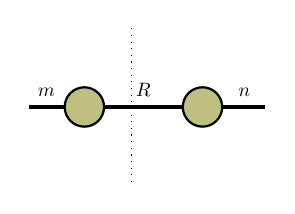
\begin{tikzpicture}[baseline=-0.5ex]
    \tikzset{tensor/.style = {minimum size = 0.5cm,shape = circle,thick,draw=black,inner sep = 0pt}, edge/.style = {thick,line width=.4mm},every loop/.style={}}
    \def\x{6}
    \def\y{0} \node[tensor,fill=green!50!red!50!white] (A) at (\x+1,\y) {$\Ab$};
    \node[tensor,fill=green!50!red!50!white] (B) at (\x+2.5,\y) {$\Bb$};
    \draw[edge] (A) -- (\x+0.3,0) node [midway,above] {\scalebox{0.7}{\dimcolor{$m$}}};
    \draw[edge] (A) -- (B)node [above,midway] {\scalebox{0.7}{\dimcolor{$R$}}};;
    \draw[edge] (B) -- (\x+3.3,\y) node [midway,above] {\scalebox{0.7}{\dimcolor{$n$}}};
    \draw[dotted] (\x+1.6,\y+1) -- (\x+1.6,\y-1);
\end{tikzpicture}\right)\leq R.$$

再考虑如下 $d_1\times d_2$ 矩阵的张量网络表示：
$$
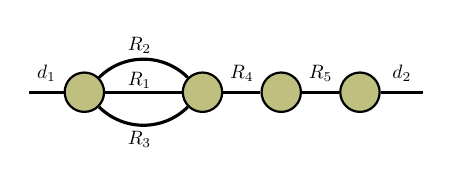
\begin{tikzpicture}[baseline=-0.5ex]
    \tikzset{tensor/.style = {minimum size = 0.5cm,shape = circle,thick,draw=black,inner sep = 0pt}, edge/.style = {thick,line width=.4mm},every loop/.style={}}
    \def\x{6}
    \def\y{0} \node[tensor,fill=green!50!red!50!white] (T) at (\x+1,\y) {$\Tt$};
    \node[tensor,fill=green!50!red!50!white] (A) at (\x+2.5,\y) {$\At$};
    \node[tensor,fill=green!50!red!50!white] (B) at (\x+3.5,\y) {$\Bb$};
      \node[tensor,fill=green!50!red!50!white] (S) at (\x+4.5,\y) {$\Sb$};
    \draw[edge] (T) -- (\x+0.3,\y)node [midway,above] {\scalebox{0.7}{\dimcolor{$d_1$}}};
     \draw[edge] (T) -- (A);
    \draw[edge] (A) -- (B)node [midway,above] {\scalebox{0.7}{\dimcolor{$R_4$}}};
    \draw[edge] (T) to [out=-45,in=-135] (A);
    \draw[edge] (T) to [out=45,in=135] (A);
    \node[draw=none] () at (\x+1.7,\y+0.15) {\scalebox{0.7}{\dimcolor{$R_1$}}};
    \node[draw=none] () at (\x+1.7,\y+0.6) {\scalebox{0.7}{\dimcolor{$R_2$}}};
    \node[draw=none] () at (\x+1.7,\y-0.6) {\scalebox{0.7}{\dimcolor{$R_3$}}};
    \draw[edge](B) -- (S) node [midway,above] {\scalebox{0.7}{\dimcolor{$R_5$}}};
    \draw[edge] (S) -- (\x+5.3,\y) node [midway,above] {\scalebox{0.7}{\dimcolor{$d_2$}}};
    \end{tikzpicture}$$
其中 $\Tt\in\RR^{d_1\times R_1\times R_2\times R_3}$，$\At\in\RR^{R_1\times R_2\times R_3\times R_4}$，$\Bb\in\RR^{R_4\times R_5}$ 且 $\Sb\in\RR^{R_5\times d_2}$。
例如，定理~\ref{thm: matricization-rank} 可用来给出上界
$$
\rank\left(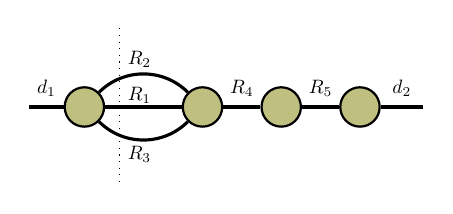
\begin{tikzpicture}[baseline=-0.5ex]
    \tikzset{tensor/.style = {minimum size = 0.5cm,shape = circle,thick,draw=black,inner sep = 0pt}, edge/.style = {thick,line width=.4mm},every loop/.style={}}
    \def\x{6}
    \def\y{0} \node[tensor,fill=green!50!red!50!white] (T) at (\x+1,\y) {$\Tt$};
    \node[tensor,fill=green!50!red!50!white] (A) at (\x+2.5,\y) {$\At$};
    \node[tensor,fill=green!50!red!50!white] (B) at (\x+3.5,\y) {$\Bb$};
      \node[tensor,fill=green!50!red!50!white] (S) at (\x+4.5,\y) {$\Sb$};
    \draw[edge] (T) -- (\x+0.3,\y)node [midway,above] {\scalebox{0.7}{\dimcolor{$d_1$}}};
     \draw[edge] (T) -- (A);
    \draw[edge] (A) -- (B)node [midway,above] {\scalebox{0.7}{\dimcolor{$R_4$}}};
    \draw[edge] (T) to [out=-45,in=-135] (A);
    \draw[edge] (T) to [out=45,in=135] (A);
    \node[draw=none] () at (\x+1.7,\y+0.15) {\scalebox{0.7}{\dimcolor{$R_1$}}};
    \node[draw=none] () at (\x+1.7,\y+0.6) {\scalebox{0.7}{\dimcolor{$R_2$}}};
    \node[draw=none] () at (\x+1.7,\y-0.6) {\scalebox{0.7}{\dimcolor{$R_3$}}};
    \draw[edge](B) -- (S) node [midway,above] {\scalebox{0.7}{\dimcolor{$R_5$}}};
    \draw[edge] (S) -- (\x+5.3,\y) node [midway,above] {\scalebox{0.7}{\dimcolor{$d_2$}}};
    \draw[dotted] (\x+1.45,\y+1) -- (\x+1.45,\y-1);
    \end{tikzpicture}\right)\leq R_1R_2R_3$$
以及
$$
\rank
\left(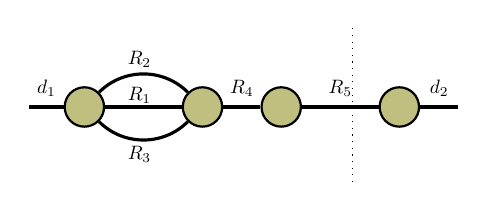
\begin{tikzpicture}[baseline=-0.5ex]
    \tikzset{tensor/.style = {minimum size = 0.5cm,shape = circle,thick,draw=black,inner sep = 0pt}, edge/.style = {thick,line width=.4mm},every loop/.style={}}
    \def\x{6}
    \def\y{0} \node[tensor,fill=green!50!red!50!white] (T) at (\x+1,\y) {$\Tt$};
    \node[tensor,fill=green!50!red!50!white] (A) at (\x+2.5,\y) {$\At$};
    \node[tensor,fill=green!50!red!50!white] (B) at (\x+3.5,\y) {$\Bb$};
      \node[tensor,fill=green!50!red!50!white] (S) at (\x+5,\y) {$\Sb$};
    \draw[edge] (T) -- (\x+0.3,\y)node [midway,above] {\scalebox{0.7}{\dimcolor{$d_1$}}};
     \draw[edge] (T) -- (A);
    \draw[edge] (A) -- (B)node [midway,above] {\scalebox{0.7}{\dimcolor{$R_4$}}};
    \draw[edge] (T) to [out=-45,in=-135] (A);
    \draw[edge] (T) to [out=45,in=135] (A);
    \node[draw=none] () at (\x+1.7,\y+0.15) {\scalebox{0.7}{\dimcolor{$R_1$}}};
    \node[draw=none] () at (\x+1.7,\y+0.6) {\scalebox{0.7}{\dimcolor{$R_2$}}};
    \node[draw=none] () at (\x+1.7,\y-0.6) {\scalebox{0.7}{\dimcolor{$R_3$}}};
    \draw[edge](B) -- (S) node [midway,above] {\scalebox{0.7}{\dimcolor{$R_5$}}};
    \draw[edge] (S) -- (\x+5.75,\y) node [midway,above] {\scalebox{0.7}{\dimcolor{$d_2$}}};
    \draw[dotted] (\x+4.4,\y+1) -- (\x+4.4,\y-1);
    \end{tikzpicture}\right)\leq R_5.
$$
最后一个例子：设 $\Gt\in\RR^{R_1\times\cdots\times R_4}$，$\Ab_1\in\RR^{R_1\times d_1}, \Ab_2\in\RR^{R_2\times d_2},\Ab_3\in\RR^{R_3\times d_3}$ 且 $\Ab_4\in\RR^{R_4\times d_4}$，并考虑张量 $\T = \Gt \times_1 \Ab_1\times_2 \Ab_2\times_3 \Ab_3\times_4 \Ab_4$。定理~\ref{thm: matricization-rank} 例如可用来给出 $\Tt$ 的第一种矩阵化的秩的上界：
$$
\rank(\Tt_{(1)}) = 
\rank\left(
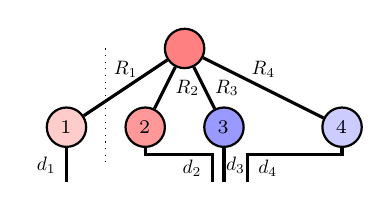
\begin{tikzpicture}[baseline=-0.5ex]
    \tikzset{tensor/.style = {minimum size = 0.5cm,shape = circle,thick,draw=black,inner sep = 0pt}, edge/.style = {thick,line width=.4mm},every loop/.style={}}
    \def\x{6}
    \def\y{0} 
    \node[tensor,fill=red!50!white] (G) at (\x+4.5,\y+1) {$\Gt$};
    \node[tensor,fill=red!20!white] (A_1) at (\x+3,\y){$\Ab_1$};
    \node[tensor,fill=red!40!white] (A_2) at (\x+4,\y){$\Ab_2$};
    \node[tensor, fill=blue!40!white] (A_3) at (\x+5,\y){$\Ab_3$};
    \node[tensor,fill=blue!20!white] (A_4) at (\x+6.5,\y){$\Ab_4$};
    \draw[edge] (G) -- (A_1) node [midway, above] {\scalebox{0.7}{\dimcolor{$R_1$}}};
    \draw[edge] (G) -- (A_2) node [midway, right] {\scalebox{0.7}{\dimcolor{$R_2$}}};
    \draw[edge] (G) -- (A_3) node [midway, right] {\scalebox{0.7}{\dimcolor{$R_3$}}};
    \draw[edge] (G) -- (A_4) node [midway, above] {\scalebox{0.7}{\dimcolor{$R_4$}}};
    \draw[edge] (A_1) -- (\x+3,\y-0.7) node [midway, left] {\scalebox{0.7}{\dimcolor{$d_1$}}};
    \draw[edge] (A_3) -- (\x+5,\y-0.7) node [midway, right=-0.11cm] {\scalebox{0.7}{\dimcolor{$d_3$}}};
    \draw[edge] (A_2) -- (\x+4,\y-0.35) -- (\x+4.85,\y-0.35) -- (\x+4.85,\y-0.7) node [midway, left] {\scalebox{0.7}{\dimcolor{$d_2$}}};
    \draw[edge] (A_4) -- (\x+6.5,\y-0.35) -- (\x+5.30,\y-0.35) -- (\x+5.30,\y-0.7) node [midway, right] {\scalebox{0.7}{\dimcolor{$d_4$}}};
    \draw[dotted](\x+3.5,\y+1)-- (\x+3.5,\y-0.5);
    \end{tikzpicture}\right)\leq R_1.
$$
\paragraph{TN 的边与和式张量。}设 $\T$ 为以 TN 给出的张量。TN 中的任意一条边，都对应一种把该张量表示为若干个与 $\T$ 同尺寸的张量之和的方式。这直接来自 TN 中边的定义。一条边表示一次收缩，而收缩就是一个求和。下面用例子说明这一概念。首先，考虑 $m\times n$ 矩阵的秩为 $R$ 的分解。TN 中的那条边对应把该矩阵表示为 $R$ 个（秩一）矩阵之和：  
$$
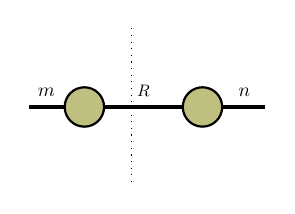
\begin{tikzpicture}[baseline=-0.5ex]
    \tikzset{tensor/.style = {minimum size = 0.5cm,shape = circle,thick,draw=black,inner sep = 0pt}, edge/.style = {thick,line width=.4mm},every loop/.style={}}
    \def\x{6}
    \def\y{0} \node[tensor,fill=green!50!red!50!white] (A) at (\x+1,\y) {$\Ab$};
    \node[tensor,fill=green!50!red!50!white] (B) at (\x+2.5,\y) {$\Bb$};
    \draw[edge] (A) -- (\x+0.3,0) node [midway,above] {\scalebox{0.7}{\dimcolor{$m$}}};
    \draw[edge] (A) -- (B)node [above,midway] {\scalebox{0.6}{\dimcolor{$R$}}};;
    \draw[edge] (B) -- (\x+3.3,\y) node [midway,above] {\scalebox{0.7}{\dimcolor{$n$}}};
    \draw[dotted] (\x+1.6,\y+1) -- (\x+1.6,\y-1);
\end{tikzpicture}
= 
\sum_{r=1}^R
\begin{tikzpicture}[baseline=-0.5ex]
    \tikzset{tensor/.style = {minimum size = 0.5cm,shape = circle,thick,draw=black,inner sep = 0pt}, edge/.style = {thick,line width=.4mm},every loop/.style={}}
    \def\x{6}
    \def\y{0} \node[tensor,fill=green!50!red!50!white] (A) at (\x+1,\y) {$\Ab$};
    \node[tensor,fill=green!50!red!50!white] (B) at (\x+2.5,\y) {$\Bb$};
    \draw[edge] (A) -- (\x+0.3,0) node [midway,above] {\scalebox{0.7}{\dimcolor{$m$}}};
    \draw[edge] (A) -- (\x+1.5,\y) node [pos=1.5] {\scalebox{0.7}{\indcolor{$r$}}};
    \draw[edge] (B) -- (\x+3.3,\y) node [midway,above] {\scalebox{0.7}{\dimcolor{$n$}}};
    \draw[edge](B) -- (\x+2,\y)node [pos=1.4] {\scalebox{0.7}{\indcolor{$r$}}};
\end{tikzpicture}
= \sum_{r=1}^R \Ab_{:,r} \Bb_{r,:} = \sum_{r=1}^R \ab_r \outprod \bb_r,
$$
其中 $\ab_r$ 为 $\Ab\in\RR^{m\times R}$ 的各列，$\bb_r$ 为 $\Bb\in\RR^{R\times n}$ 的各行。

类似地，表示矩阵的迹的那个 TN 中唯一的边，对应于把这个 TN（它是一个标量）写成若干标量（矩阵的对角元）之和，设 $\Ab\in\RR^{d\times d}$：
$$\begin{tikzpicture}[baseline=\baseline]
    \tikzset{tensor/.style = {minimum size = 0.5cm,shape = circle,thick,draw=black,inner sep = 0pt}, edge/.style = {thick,line width=.4mm},every loop/.style={}}
    \def\y{0}
    \def\x{0}
    \node[tensor,fill=red!50!white] (A) at (\x,\y+0.2){\scalebox{0.85}{$\Ab$}};
    \draw[edge] (A) to [out=-20,in=-160, distance=1.35cm] (A);
    \draw[dotted] (\x-0.15,\y-0.1) -- (\x-0.15,\y-0.8);
    \node[draw=none] () at (\x,\y-0.4) {\scalebox{0.7}{\dimcolor{$d$}}};
\end{tikzpicture}\hspace{-0.7cm}
=
\sum_{i=1}^d\left(
\begin{tikzpicture}[baseline=\baseline]
    \tikzset{tensor/.style = {minimum size = 0.5cm,shape = circle,thick,draw=black,inner sep = 0pt}, edge/.style = {thick,line width=.4mm},every loop/.style={}}
    \def\y{0}
    \def\x{0}
    \node[tensor,fill=red!50!white] (A) at (\x,\y){\scalebox{0.85}{$\Ab$}};
     \draw[edge] (\x-0.25,\y) to [out=110,in=60, distance=0.1cm] (\x-0.6,\y-0.2);    
    \draw[edge] (\x+0.25,\y) to [out=110,in=60, distance=0.1cm] (\x+0.6,\y-0.2); 
    \node[draw=none] () at (\x+0.7,\y-0.25) {\scalebox{0.7}{\indcolor{$i$}}};
    \node[draw=none] () at (\x-0.7,\y-0.25) {\scalebox{0.7}{\indcolor{$i$}}};
    \end{tikzpicture}\right)=\sum_{i=1}^d\Ab_{ii}.
    $$
现在考虑一个更有趣的例子：
$$\begin{tikzpicture}[baseline=\baseline]
    \tikzset{tensor/.style = {minimum size = 0.5cm,shape = circle,thick,draw=black,inner sep = 0pt}, edge/.style = {thick,line width=.4mm},every loop/.style={}}
    \def\y{0}
    \def\x{0}
    \node[tensor,fill=red!50!white] (A) at (\x,\y+0.5){\scalebox{0.85}{$\Ab$}};
    \node[tensor,fill=red!50!white] (B) at (\x,\y-0.5){\scalebox{0.85}{$\Bb$}};
    \draw[edge](A)--(B)node [midway, right] {\scalebox{0.7}{\dimcolor{$R$}}};
    \draw[edge](A) -- (\x+0.5,\y+0.5)--(\x+0.5,\y)--(\x+1,\y)node [midway, above] {\scalebox{0.7}{\dimcolor{$n$}}};
    \draw[edge](A) -- (\x-0.5,\y+0.5)--(\x-0.5,\y)--(\x-1,\y)node [midway, above] {\scalebox{0.7}{\dimcolor{$m$}}};
    \draw[edge](B) -- (\x+0.5,\y-0.5)--(\x+0.5,\y-0.1)--(\x+1,\y-0.1)node [midway, below] {\scalebox{0.7}{\dimcolor{$q$}}};
    \draw[edge](B) -- (\x-0.5,\y-0.5)--(\x-0.5,\y-0.1)--(\x-1,\y-0.1)node [midway, below] {\scalebox{0.7}{\dimcolor{$p$}}};
    \end{tikzpicture}.$$
这个 TN 中的边对应于一种表达矩阵的方式：把该 TN 所表示的矩阵写成若干矩阵之和：
$$\begin{tikzpicture}[baseline=\baseline]
    \tikzset{tensor/.style = {minimum size = 0.5cm,shape = circle,thick,draw=black,inner sep = 0pt}, edge/.style = {thick,line width=.4mm},every loop/.style={}}
    \def\y{0}
    \def\x{0}
    \node[tensor,fill=red!50!white] (A) at (\x,\y+0.5){\scalebox{0.85}{$\Ab$}};
    \node[tensor,fill=red!50!white] (B) at (\x,\y-0.5){\scalebox{0.85}{$\Bb$}};
    \draw[edge](A)--(B)node [midway, right] {\scalebox{0.7}{\dimcolor{$R$}}};
    \draw[edge](A) -- (\x+0.5,\y+0.5)--(\x+0.5,\y)--(\x+1,\y)node [midway, above] {\scalebox{0.7}{\dimcolor{$n$}}};
    \draw[edge](A) -- (\x-0.5,\y+0.5)--(\x-0.5,\y)--(\x-1,\y)node [midway, above] {\scalebox{0.7}{\dimcolor{$m$}}};
    \draw[edge](B) -- (\x+0.5,\y-0.5)--(\x+0.5,\y-0.1)--(\x+1,\y-0.1)node [midway, below] {\scalebox{0.7}{\dimcolor{$q$}}};
    \draw[edge](B) -- (\x-0.5,\y-0.5)--(\x-0.5,\y-0.1)--(\x-1,\y-0.1)node [midway, below] {\scalebox{0.7}{\dimcolor{$p$}}};
    \draw[dotted](\x+0.35,\y+0.15) -- (\x-0.35,\y+0.15);
    \end{tikzpicture}
    =
    \sum_{r=1}^R\begin{tikzpicture}[baseline=\baseline]
    \tikzset{tensor/.style = {minimum size = 0.5cm,shape = circle,thick,draw=black,inner sep = 0pt}, edge/.style = {thick,line width=.4mm},every loop/.style={}}
    \def\y{0}
    \def\x{0}
    \node[tensor,fill=red!50!white] (A) at (\x,\y+1){\scalebox{0.85}{$\Ab$}};
    \node[tensor,fill=red!50!white] (B) at (\x,\y-1){\scalebox{0.85}{$\Bb$}};
    \draw[edge](A) -- (\x,\y+0.45)node [pos=1.4]{\scalebox{0.7}{\indcolor{$r$}}};
    \draw[edge](B) -- (\x,\y-0.45)node [pos=1.3]{\scalebox{0.7}{\indcolor{$r$}}};
    \draw[edge](A) -- (\x+0.5,\y+1)--(\x+0.5,\y)--(\x+1,\y)node [midway, above] {\scalebox{0.7}{\dimcolor{$n$}}};
    \draw[edge](A) -- (\x-0.5,\y+1)--(\x-0.5,\y)--(\x-1,\y)node [midway, above] {\scalebox{0.7}{\dimcolor{$m$}}};
    \draw[edge](B) -- (\x+0.5,\y-1)--(\x+0.5,\y-0.1)--(\x+1,\y-0.1)node [midway, below] {\scalebox{0.7}{\dimcolor{$q$}}};
    \draw[edge](B) -- (\x-0.5,\y-1)--(\x-0.5,\y-0.1)--(\x-1,\y-0.1)node [midway, below] {\scalebox{0.7}{\dimcolor{$p$}}};
    \end{tikzpicture}
    =
    \sum_{r=1}^R\Ab_r\kron\Bb_r.$$
由此可见，这个 TN 对应的正是 Kronecker 积之和！ 
\paragraph{张量、多重线性映射与多项式。}
可以把张量看作\emph{多重线性映射的表示}，其含义与矩阵表示线性映射完全相同。回顾一下，矩阵 $\Ab\in\RR^{m\times n}$ 通过 $\xb\mapsto \Ab\xb$ 表示一个线性映射 $\RR^n\to\RR^m$。用张量网络记法，这就是
$$
\yb = \Ab\xb
=
\begin{tikzpicture}[baseline=-0.5ex]
    \tikzset{tensor/.style = {minimum size = 0.5cm,shape = circle,thick,draw=black,inner sep = 0pt},
             edge/.style   = {thick,line width=.4mm},every loop/.style={}}
    \def\x{0}\def\y{0}
    \node[tensor,fill=red!50!white] (A) at (\x,\y){$\Ab$};
    \node[tensor,fill=blue!20!white] (x) at (\x+1,\y){$\xb$};
    \draw[edge] (A) -- (x) node [midway,above]{\scalebox{0.7}{\dimcolor{$n$}}};
    \draw[edge] (A) -- (\x-1,\y) node [midway,above]{\scalebox{0.7}{\dimcolor{$m$}}};
\end{tikzpicture}
\in\RR^{m}.
$$
线性是指对一切 $\alpha,\beta\in\RR$ 与 $\xb,\zb\in\RR^n$ 都有 $\Ab(\alpha \xb+\beta \zb)=\alpha \Ab\xb+\beta \Ab\zb$。当映射\emph{对每个自变量分别线性}时，张量便是其自然推广。具体地说，一个 $N$ 阶张量 $\Tt\in\RR^{d_1\times\cdots\times d_N}$ 定义了一个映射：它接受 $N$ 个输入向量，并沿所有模收缩而给出一个标量：
$$
f(\xb^{(1)},\dots,\xb^{(N)})
:= \langle \Tt,\ \xb^{(1)}\outprod \cdots \outprod \xb^{(N)}\rangle
=
\sum_{i_1=1}^{d_1}\cdots\sum_{i_N=1}^{d_N}\Tt_{i_1\cdots i_N}\,\xb^{(1)}_{i_1}\cdots \xb^{(N)}_{i_N}.
$$
该映射是\emph{多重线性}的：固定其余向量时，它对每个 $\xb^{(k)}$ 都是线性的。在张量网络图中，这就是
\[
f(\ab,\bb,\dots,\zb)
=
\begin{tikzpicture}[baseline=2ex]
    \tikzset{tensor/.style = {minimum size = 0.5cm,shape = circle,thick,draw=black,inner sep = 0pt},
             edge/.style   = {thick,line width=.4mm},
             every loop/.style={}}
    \def\x{0}\def\y{0}

    \node[tensor,fill=green!50!red!50!white] (T) at (\x,\y+0.8){$\Tt$};

    \node[tensor,fill=blue!20!white] (a) at (\x-1.2,\y){$\ab$};
    \node[tensor,fill=blue!20!white] (b) at (\x-0.5,\y){$\bb$};
    \node[draw=none] (dots) at (\x+0.5,\y){$\cdots$};
    \node[tensor,fill=blue!20!white] (z) at (\x+1.2,\y){$\zb$};

    \draw[edge] (T) -- (a) node [near end,above]{\scalebox{0.7}{\dimcolor{$d_1\ $}}};
    \draw[edge] (T) -- (b) node [near end,right]{\scalebox{0.7}{\dimcolor{$d_2$}}};
    \draw[edge] (T) -- (z) node [near end,above]{\scalebox{0.7}{\dimcolor{$d_N$}}};
\end{tikzpicture}
\in\RR,
\]
其中 $\ab, \bb,\cdots,\zb\in\RR^d$。
若留出一条腿不作收缩，便得到一个\emph{向量值}多重线性映射。例如，若 $\Tt\in\RR^{d_1\times\cdots\times d_N \times p}$，则除最后一个模之外对所有的模收缩，就定义了一个输出为 $p$ 维向量的多重线性映射：
$$
f(\ab,\bb,\dots,\zb)
=
\begin{tikzpicture}[baseline=2ex]
    \tikzset{tensor/.style = {minimum size = 0.5cm,shape = circle,thick,draw=black,inner sep = 0pt},
             edge/.style   = {thick,line width=.4mm},
             every loop/.style={}}
    \def\x{0}\def\y{0}

    \node[tensor,fill=green!50!red!50!white] (T) at (\x,\y+0.8){$\Tt$};

    \node[tensor,fill=blue!20!white] (a) at (\x-1.2,\y){$\ab$};
    \node[tensor,fill=blue!20!white] (b) at (\x-0.5,\y){$\bb$};
    \node[draw=none] (dots) at (\x+0.5,\y){$\cdots$};
    \node[tensor,fill=blue!20!white] (z) at (\x+1.2,\y){$\zb$};

    \draw[edge] (T) -- (a) node [near end,above]{\scalebox{0.7}{\dimcolor{$d_1\ $}}};
    \draw[edge] (T) -- (b) node [near end,right]{\scalebox{0.7}{\dimcolor{$d_2$}}};
    \draw[edge] (T) -- (z) node [near end,above]{\scalebox{0.7}{\dimcolor{$d_N$}}};
    \draw[edge] (T) -- (\x,\y+1.6) node [midway,right]{\scalebox{0.7}{\dimcolor{$p$}}};
\end{tikzpicture}
\in\RR^p.
$$

\vspace{0.2cm}
\noindent
这就把张量直接与\emph{多元多项式}联系了起来。上面的标量映射
\[
f(\xb^{(1)},\dots,\xb^{(N)})=\sum_{i_1,\dots,i_N}\Tt_{i_1\cdots i_N}\,\xb^{(1)}_{i_1}\cdots \xb^{(N)}_{i_N},
\]
是关于各向量分量的多项式，并且是\emph{多重线性}的：每个变量出现的次数至多为一（就每一组变量 $\xb^{(k)}$ 而言如此）。在一个重要的特殊情形中，所有输入都是\emph{同一个}向量 $\xb\in\RR^{d}$，而 $\Tt\in\RR^{d\times\cdots\times d}$ 有 $N$ 个模，此时收缩
\[
\begin{tikzpicture}[baseline=2ex]
    \tikzset{tensor/.style = {minimum size = 0.5cm,shape = circle,thick,draw=black,inner sep = 0pt},
             edge/.style   = {thick,line width=.4mm},
             every loop/.style={}}
    \def\x{0}\def\y{0}

    \node[tensor,fill=green!50!red!50!white] (T) at (\x,\y+0.8){$\Tt$};

    \node[tensor,fill=blue!20!white] (a) at (\x-1.2,\y){$\xb$};
    \node[tensor,fill=blue!20!white] (b) at (\x-0.5,\y){$\xb$};
    \node[draw=none] (dots) at (\x+0.5,\y){$\cdots$};
    \node[tensor,fill=blue!20!white] (z) at (\x+1.2,\y){$\xb$};

    \draw[edge] (T) -- (a) node [midway,left]{\scalebox{0.7}{\dimcolor{$d\ $}}};
    \draw[edge] (T) -- (b) node [near end,right]{\scalebox{0.7}{\dimcolor{$d$}}};
    \draw[edge] (T) -- (z) node [midway,right]{\scalebox{0.7}{\dimcolor{$\ d$}}};
\end{tikzpicture}
= \Tt \ttm{1}\xb \ttm{2}\xb \cdots \ttm{N}\xb
=
\sum_{i_1,\dots,i_N}\Tt_{i_1\cdots i_N}\,\xb_{i_1}\cdots \xb_{i_N} \in \RR.
\]
是一个 $N$ 次\emph{齐次}多元多项式（每个单项式的总次数恰为 $N$）。张量的分量恰好是这一多项式在单项式基 $(\xb_{i_1}\cdots \xb_{i_N})_{i_1,\cdots,i_N}$ 下的系数。

反之，若把 $(N+1)$ 阶张量 $\Tt\in\RR^{ d\times\cdots\times d \times p}$ 与 $N$ 份 $\xb\in\RR^d$ 收缩，并让最后一条腿保持自由，就得到一个向量值的齐次多项式映射 $\RR^d\to\RR^m$：
\[
p(\xb) = \Tt \ttm{1}\xb \ttm{2}\xb\cdots \ttm{N}\xb \in\RR^{p}.
\]

\vspace{0.2cm}
\noindent
最后，\emph{非齐次}多项式可以用一个小技巧得到：\emph{在输入向量末尾添上一个常数 $1$}。设 $\xb\in\RR^d$，并定义增广向量 $\tilde{\xb} =\begin{bmatrix}\xb\\1\end{bmatrix}\in\RR^{d+1}$。若 $\widetilde{\Tt}\in\RR^{(d+1)\times\cdots\times(d+1)}$ 是一个 $N$ 阶张量，则
\[
\tilde{p}(\xb)
:=
\widetilde{\Tt} \ttm{1}\tilde{\xb}\ttm{2}\tilde{\xb}\cdots\ttm{N}\tilde{\xb},
\]
是 $\xb$ 的不超过 $N$ 次的多项式（某些因子会取到最后一个坐标，也就是常数 $1$，从而降低相应单项式的次数）。换句话说，增广变量 $(x_1,\dots,x_d,1)$ 的一个齐次张量多项式，就紧凑地表示了 $(x_1,\dots,x_d)$ 的一般多元多项式。这一观点在实践中尤为有用：只需给每个模添加一个额外的维度并把它固定为 $1$，就能用与齐次情形相同的收缩机制来处理偏置项与低次交互项。  
